\documentclass[12pt]{article}
\usepackage[papersize={8.5in,11in}, margin = 1in]{geometry}
\usepackage[utf8]{inputenc}
\usepackage{setspace}
\usepackage{amssymb}
\usepackage{amsmath}
\usepackage{physics}
\usepackage{fancyhdr}
\usepackage{enumitem}
\usepackage{lastpage}
\usepackage[none]{hyphenat}%%%%
\usepackage[scr]{rsfso}
\usepackage[dvipsnames]{xcolor}
\usepackage{graphicx}
\usepackage{caption}
\captionsetup{font=footnotesize}
\usepackage{subcaption}
\usepackage{float}
\usepackage{listings}
\usepackage{titlesec}
\usepackage{algorithm}
\usepackage{algpseudocode}
\usepackage{placeins}
\usepackage{newtxtext,newtxmath}
\usepackage{ragged2e}
\usepackage{multirow}
\usepackage{url}
\bibliographystyle{unsrt}

\titleformat{\section}[block]{\normalfont\Large\bfseries}{\thesection}{1em}{}
\titlespacing{\section}{0pt}{*1.5}{0pt}
\titlespacing{\subsection}{0pt}{*0.75}{0pt}

\usepackage{hyperref}
\hypersetup{
    colorlinks=true,
    linktoc=all,
    linkcolor=teal,
    urlcolor=teal,
    citecolor=teal,
}
\graphicspath{{pics/}}

% because khushant's title page is wonky -BA
\usepackage{atbegshi}% http://ctan.org/pkg/atbegshi
% \AtBeginDocument{\AtBeginShipoutNext{\AtBeginShipoutDiscard}}

% for codeblocks
\definecolor{codegreen}{rgb}{0,0.6,0}
\definecolor{codegray}{rgb}{0.5,0.5,0.5}
\definecolor{codepurple}{rgb}{0.58,0,0.82}
\definecolor{backcolour}{rgb}{0.95,0.95,0.92}

\lstdefinestyle{mystyle}{
    backgroundcolor=\color{backcolour},   
    commentstyle=\color{codegreen},
    keywordstyle=\color{magenta},
    numberstyle=\tiny\color{codegray},
    stringstyle=\color{codepurple},
    basicstyle=\ttfamily\footnotesize,
    breakatwhitespace=false,         
    breaklines=true,                 
    captionpos=b,                    
    keepspaces=true,                 
    numbers=left,                    
    numbersep=5pt,                  
    showspaces=false,                
    showstringspaces=false,
    showtabs=false,                  
    tabsize=2
}

\lstset{style=mystyle}

\pagestyle{fancy}
\fancyhead[L]{\small University of Pennsylvania \\ MEAM 6240 - Distributed Robotics}
\fancyhead[R]{\small Benjamin Aziel and Jason Chen \\ \today}
\fancyfoot[C]{Page \thepage\ of \pageref{LastPage}} 
\fancyfoot[C]{Page \thepage \hspace{1pt} of \pageref{LastPage}}

\newcommand{\Volume}{{\ooalign{\hfil$V$\hfil\cr\kern0.08em--\hfil\cr}}}
\begin{document}

% https://www.lifewire.com/text-alignment-tips-1074943
% i'm very biased towards flushleft. sorry justify fans

\thispagestyle{empty}
\newcommand{\titleName}{Performance Analysis of the Boids Algorithm in Coverage Scenarios\\[.4cm]
\textmd{\LARGE MEAM 6240 - Distributed Robotics}}
\begin{titlepage} 
	\newcommand{\HRule}{\rule{\linewidth}{0.5mm}}
	\center
	\textsc{\LARGE University of Pennsylvania}\\[2.5cm] 
	{\color{black} \HRule\\[0.4cm]}
	{\huge\bfseries \titleName}\\[0.4cm] 
	{\color{black} \HRule\\[0.4cm]}
	\begin{minipage}{0.4\textwidth}
		\begin{flushleft}
			\large
			\textit{Authors:}\\
            \textsc{Benjamin Aziel} \\
            \textsc{Jason Chen}\\
            \text{ }\\
		\end{flushleft}
	\end{minipage}
	~
	\begin{minipage}{0.4\textwidth}
		\begin{flushright}
			\large
			\textit{Professor:}\\
			\textsc{Cynthia Sung}\\ 
            \text{ }\\
            \text{ }\\
		\end{flushright}
	\end{minipage}
	\vfill

    \vfill
	{\large Last Updated: \today}
	\vfill
%----------------------------------------------------------------------------------------
\end{titlepage}

\fancypagestyle{tocstyle}{
    \fancyhf{} 
    \renewcommand{\footrulewidth}{0pt} 
    \renewcommand{\headrulewidth}{0.4pt} 
}

\thispagestyle{tocstyle}
\tableofcontents
\pagenumbering{gobble}
\pagebreak

\abovedisplayskip=6pt
\belowdisplayskip=0pt
\abovedisplayshortskip=0pt
\belowdisplayshortskip=0pt

\pagenumbering{arabic}
\setcounter{page}{1}

\setlength{\parindent}{0pt}
\setlength{\parskip}{0.25em}
\section*{Abstract}

The objective of this project is to implement and analyze the boids model for flocking behavior, with a focus on optimizing its effectiveness for coverage tasks through systematic tuning of key behavioral parameters. By adjusting the core gains that govern alignment, cohesion, and separation, the same underlying framework can yield a wide spectrum of emergent group dynamics, ranging from tight, cohesive flocking to deliberate spatial dispersion. The implementation explores the practical applications of these behaviors for distributed robotics systems, with quantitative exploration analysis across various parameter configurations and environmental scenarios.

\section{Introduction}

Collective behavior is a well-documented phenomenon in natural systems, observable in bird flocks, fish schools, and herds of terrestrial animals. These systems exhibit coordinated, large-scale movement patterns that appear to emerge from simple local interactions between individuals. Craig Reynolds formalized this concept with the boids model in his 1986 paper ``\emph{Flocks, Herds, and Schools: A Distributed Behavior Model}'' \cite{reynolds1987flocks}. This project builds on that framework by reimplementing Reynolds' original algorithm and extending it for use in robotic exploration tasks, focusing on performance optimization through parameter tuning.

The boids model is governed by three canonical local rules: separation, alignment, and cohesion, described in detail in Section 2.

\begin{figure}[h!]
    \centering
    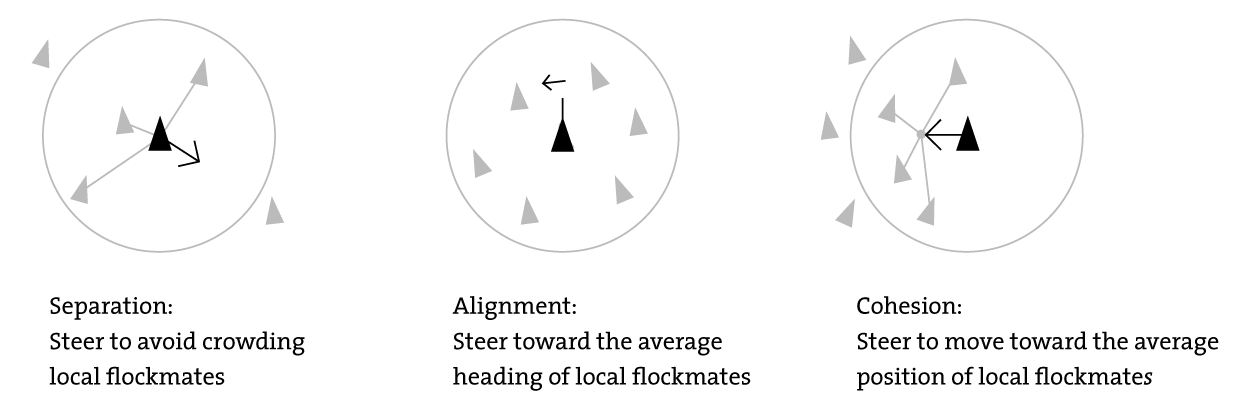
\includegraphics[width=0.7\linewidth]{force_diagram.png}
    \caption{Illustration of local force computations for a single boid \(i\). Cohesion pulls the agent toward neighbors, alignment encourages matching velocity, and separation pushes the agent away from close agents. Obstacle and wall avoidance forces are repulsive and operate independently. Source: \cite{martinez2023boids}}
    \label{fig:force_diagram}
  \end{figure}

Despite their simplicity, these rules give rise to complex, decentralized group dynamics without global coordination. This makes the model highly relevant to applications such as swarm robotics, where systems must be scalable, robust to individual failures, and capable of adapting to unknown or dynamic environments.

In this work, the boids model is repurposed for robotic coverage. Rather than merely replicating natural flocking behavior, the focus is on optimizing behavioral parameters, i.e., the weightings of separation, alignment, and cohesion, to achieve task-oriented objectives. The goal is to maximize coverage efficiency, defined by metrics such as area coverage and dispersion uniformity.

The simulator used for optimization also includes options for real-time parameter adjustment and obstacle avoidance capabilities. Systematic experimentation across the gain space enables identification of configurations that strike a balance between coordinated movement and spatial dispersion to allow for more effective coverage.

\section{Simulation Framework}

To support systematic exploration and parameter optimization, a custom boids-based simulator was developed using PyGame, a Python library for 2D graphics and user interaction. The simulator can be seen in Figure \ref{fig:boids_sim}. The simulator supports both interactive and headless modes, with real-time visualization and batch optimization. Full implementation details are described in Section 3.3.

\begin{figure}[h!]
    \centering
    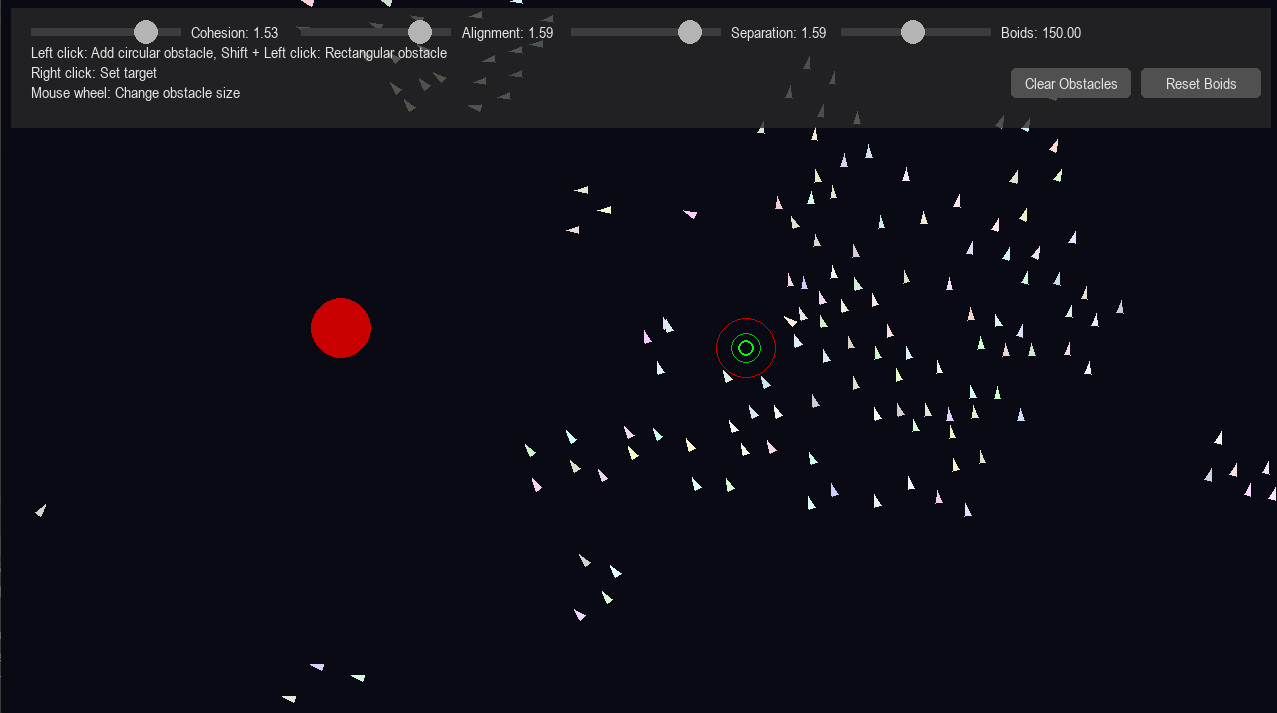
\includegraphics[width=0.7\linewidth]{boids_sim.png}
    \caption{Interactive simulation of the Boids model during runtime. A red circle indicates a user-placed obstacle, while the green target marker represents the global goal toward which boids are directed. The UI at the top enables real-time adjustment of behavioral gains for cohesion, alignment, and separation, as well as boid count and obstacle management.}
    \label{fig:boids_sim}
  \end{figure}

The architecture is modular, with the following components:
\begin{itemize}[nosep]
    \item \texttt{boid}, which implements the \texttt{Boid} class with core flocking behaviors
    \item \texttt{obstacles}, which defines obstacle representations and collision management
    \item \texttt{ui}, which handles rendering and interactive controls
    \item \texttt{simulation}, which coordinates all system components and updates
    \item \texttt{main}, which initializes the boids and launches the simulation
\end{itemize}

The simulator implements the three canonical behaviors central to the boids model: separation, alignment, and cohesion. Each of these arises from decentralized interaction rules, in which agents make steering decisions based on local sensing. Specifically, each boid perceives only other agents within a fixed perception radius and within a field-of-view cone, mimicking limited sensing capabilities found in physical agents.

The mathematical model implemented in this work is adapted from the original Boids formulation by Reynolds~\cite{reynolds1987flocks} and formalized based on principles presented in the Distributed Robotics course notes by Sung~\cite{sung2025distributed}. Within its perceived neighborhood \(\mathcal{N}_i(t)\), boid \(i\) computes a set of behavioral forces that determine its instantaneous acceleration. Let \(x_i \in \mathbb{R}^2\) denote the position of boid \(i\), and \(\dot{x}_i \in \mathbb{R}^2\) its velocity at time \(t\). These quantities are used to define the core behavioral forces governing flocking.

The collision avoidance force \(f_{\text{col}}\) pushes the agent away from nearby flockmates to reduce local density. It is computed as a repulsive sum of displacement vectors from all neighbors in the visible neighborhood, scaled by a gain \(k_{\text{col}}\):
\begin{equation} f_\text{col} = k_\text{col} \sum_{j \in \mathcal{N}_i(t)} (x_i - x_j) \end{equation}

For alignment and cohesion, the vector sum is normalized by the number of neighbors to compute the local average velocity and position, respectively; this ensures that the resulting steering direction reflects the group's overall tendency rather than being biased by the number or density of nearby agents. The alignment force \(f_\text{ali}\) encourages velocity matching with nearby flockmates. It is defined as the difference between the average velocity of visible neighbors and the agent’s current velocity, scaled by a gain \(k_\text{ali}\): 
\begin{equation} f_\text{ali} = k_\text{ali} \left( \frac{1}{|\mathcal{N}_i(t)|} \sum_{j \in \mathcal{N}_i(t)} \dot{x}_j - \dot{x}_i \right) \end{equation}

The cohesion force \(f_\text{coh}\) attracts the agent toward the center of mass of its neighborhood. It is computed as the displacement from the agent to the average position of its neighbors, scaled by \(k_\text{coh}\): 
\begin{equation} f_\text{coh} = k_\text{coh} \left( \frac{1}{|\mathcal{N}_i(t)|} \sum_{j \in \mathcal{N}_i(t)} x_j - x_i \right) \end{equation}

In addition to these flocking behaviors, agents also respond to environmental geometry. The obstacle avoidance force \(f_{\text{obs}}\) is computed as a sum of repulsive vectors from nearby obstacle locations \(o_m\), scaled by inverse squared distance to produce a smooth avoidance behavior. A small constant \(\varepsilon > 0\) is added to the denominator to avoid singularities:
\begin{equation} f_\text{obs} = \sum_m \frac{x_i - o_m}{\left( \|x_i - o_m\| + \varepsilon \right)^2} \end{equation}

A special case of this is the wall repulsion force \(f_\text{wall}\), which keeps agents within the rectangular simulation bounds. This is treated as implicit obstacle repulsion from the domain boundaries of width \(W\) and height \(H\): \begin{equation} f_\text{wall} = k_\text{wall} \begin{bmatrix}
\frac{1}{x_i + \varepsilon} - \frac{1}{W - x_i + \varepsilon} \\
\frac{1}{y_i + \varepsilon} - \frac{1}{H - y_i + \varepsilon}
\end{bmatrix} \end{equation}

The simulator also supports direct user interaction to dynamically configure the environment during runtime. Users can place obstacles in the environment using mouse input. The simulator currently supports both circular and rectangular obstacle types. This system enables the creation of realistic and heterogeneous test environments without modifying source code. When the user clicks in the PyGame simulation window while in obstacle-placement mode, a new obstacle is instantiated at the cursor location and added to the environment. This mechanism allows rapid prototyping of complex environments, such as cluttered indoor scenes, facilitating evaluation of the flock's navigational agility and adaptability under different spatial constraints.

In addition to environmental modification, the simulator includes a targeting mechanism that enables the user to assign a global heading objective to the flock. When enabled, a target point (typically set via mouse click) is rendered on the simulation display. Each boid will then attempt to steer towards this point using a dedicated target-seeking behavior.

\sloppypar
To realistically simulate physical constraints, a prioritized acceleration framework was implemented. Each boid has a limited total acceleration budget per timestep. When multiple behavioral directives are active, higher-priority behaviors consume available acceleration first. Lower-priority behaviors are only applied if residual capacity remains. The prioritization hierarchy is as follows, from highest to lowest:
\begin{equation}\text{Obstacle Avoidance} \to \text{Separation} \to \text{Alignment} \to \text{Cohesion} \to \text{Target Seeking}\end{equation}

Each force is applied sequentially and scaled to fit within the remaining acceleration budget. If the magnitude of a force exceeds the available capacity, it is truncated proportionally. Once the budget is depleted, all subsequent forces in the priority list are skipped for that timestep. This leads to behavior that dynamically adapts to situational demands, closely resembling real-world decision making under physical constraints. Compared to traditional weighted vector summation, this method provides a more biologically plausible and computationally realistic behavior model.

\section{Coverage Task and Optimization}

To evaluate the utility of the boids model for distributed exploration, a coverage task was defined in which agents aim to maximize the percentage of a 2D environment they collectively traverse. The objective is to identify gain configurations (specifically the cohesion, alignment, and separation gains) that optimize coverage while preserving desirable collective behaviors such as dispersion, obstacle negotiation, and responsiveness.

\subsection{Task Definition and Environments}

Four distinct environments, as shown in Figure \ref{fig:boids_maps} were developed to assess the generality of exploration performance across varying spatial constraints:
\begin{itemize}[nosep]
    \item \textbf{Dense Cafeteria Map}: A highly cluttered environment with tightly packed tables and surrounding chairs, which stresses local collision avoidance
    \item \textbf{Cafeteria Map}: A cluttered layout composed of circular (tables) and square (chairs) obstacles arranged in a semi-structured environment, simulating realistic indoor navigation challenges
    \item \textbf{Narrow Corridor}: A scenario containing a bottleneck, requiring agents to transition through a constrained passage, which tests local reformation and dispersion under topological stress
    \item \textbf{Empty Map}: An unobstructed arena used as a baseline for evaluating pure flocking behavior and maximum dispersion potential
\end{itemize}

\begin{figure}[h!]
    \centering
    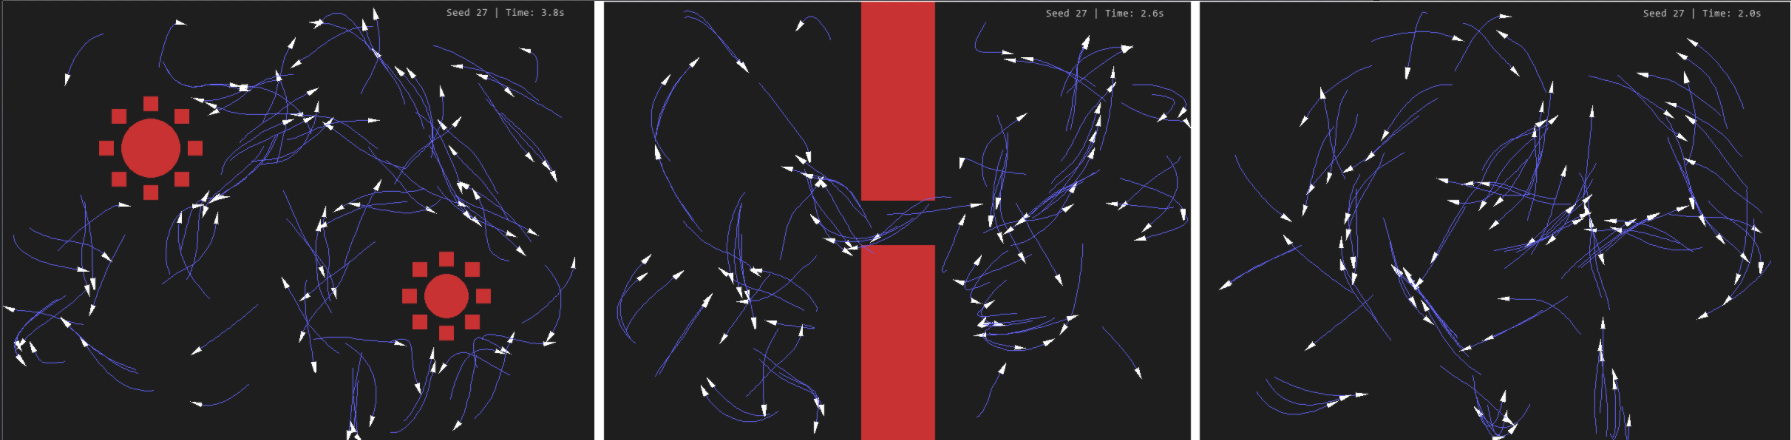
\includegraphics[width=\linewidth, trim=0 0 0 35, clip]{boids_maps.png}
    \caption{Evaluation environments used for testing: dense cafeteria map, cafeteria map, narrow corridor, and empty map, from left to right. Each layout presents different navigational challenges and constraints.}
    \label{fig:boids_maps}
  \end{figure}

\subsection{Coverage Metrics}

The coverage percentage is defined:
\begin{equation}\text{Coverage} = \frac{\text{Unique visited pixels}}{\text{Total traversable pixels}} \times 100\%\end{equation}

This metric captures the proportion of the environment that has been physically traversed by at least one agent during the simulation. It is particularly well-suited for decentralized robotic coverage tasks, where the objective is to ensure that all accessible regions are visited, regardless of the specific trajectories taken. Unlike path-efficiency or goal-reaching metrices, coverage emphasizes dispersion and collective reach, making it ideal for applications such as search-and-rescue and environmental monitoring, where spatial redundancy should be minimized.

A fixed-radius disk of 2 pixels around each agent is used to approximate the agent's effective footprint per frame. This provides a tractable and uniform discretization for coverage accumulation, while abstracting away platform-specific factors like body geometry. The 2-pixel radius was empirically selected to balance between over-counting due to overlapping footprints and under-sampling of narrow features in the environment.


\subsection{Simulation Details}

To support both visualization during development and efficient batch evaluation during optimization, two simulation modes were implemented:

\begin{enumerate}[nosep]
    \item \textbf{Interactive Mode}: Used during development and for real-time demonstrations. This version includes full graphical rendering, mouse interaction for obstacle placement and target setting, and real-time parameter adjustment via sliders. It is primarily used to observe qualitative behaviors, test hypotheses, generate illustrative figures, and debug.
    \item \textbf{Headless Mode}: A stripped-down version of the simulator designed for speed and reproducibility. This version runs without rendering or user input. It supports parallel evaluation of gain vectors across multiple random seeds using Python's \texttt{multiprocessing} module. It is the default mode used for parameter sweeps and data collection.
\end{enumerate}

The most notable change for optimization is the complete removal of graphics and visualization routines. Unlike the interactive simulation, which runs within a PyGame window and provides real-time visual feedback, the optimization version runs entirely headless. No rendering, frame drawing, or event handling is performed. This allows for simulations to be executed in parallel using the \texttt{multiprocessing} module, significantly accelerating the parameter search. Each simulation job is defined as a unique pair of a sampled gain vector and a fixed random seed. These jobs are distributed across worker processes to evaluate parameter configurations in parallel, significantly reducing overall runtime.

Additionally, user interaction capabilities are stripped away. The optimization simulation does not support real-time obstacle placement or target assignment. Instead, each environment is instantiated procedurally at the start of each trial using one of the three aforementioned predefined layouts.

Real-time parameter adjustment via sliders is replaced with randomized sampling of gain vectors within predefined bounds. Each gain vector is evaluated in a self-contained trial, allowing for fully automated search over the parameter space.

Each trial begins by instantiating \(N\) boids, each with randomized initial positions and velocities. Initial velocities are oriented uniformly at random in \([0, 2\pi)\) radians and scaled by the maximum speed. A validation step ensures that no boid is initialized within an obstacle's geometry. Each simulation runs for a fixed duration of 60 seconds, and the system updates at 60 frames per second, totaling 3600 simulation steps per trial. Behavioral forces are computed as described in Section 2 and used to update each agent’s state.

In the optimization code, the simulation domain is adjusted into an 800 \(\times\) 600 pixel grid. This reduced resolution was chosen to balance coverage fidelity with computational efficiency, allowing for faster execution of large numbers of parallel trials without compromising the spatial complexity of the environment. All environmental features and agent initializations are fully deterministic given a fixed random seed, ensuring repeatable and unbiased performance measurements. For each gain vector, the simulation is evaluated across three random seeds (27, 729, and 4913). These seeds are used to initialize the PRNG for placement, velocity, and repeated sampling if the initial sample was rejected due to obstacle conflict.

\subsection{Optimization Process}

To identify high-performing behavior parameters, we conducted a systematic random search over the space of flocking gains. Specifically, each gain vector consisted of the tuple \((k_\text{coh}, k_\text{ali}, k_\text{col})\). For each vector, coverage performance was evaluated under fixed environmental and simulation conditions.

The gain values were sampled uniformly from the following bounded intervals:
\begin{itemize}[nosep]
    \item \(k_\text{coh} \in [0.0, 0.5]\)
    \item \(k_\text{ali} \in [0.0, 0.1]\)
    \item \(k_\text{col} \in [0.0, 0.5]\)
\end{itemize}

Initially, the alignment gain was sampled over a broader range \([0.0, 0.5]\), consistent with the other parameters. The initial uniform sampling cube of \([0.0, 0.5]^3\) was chosen for an exploratory baseline, to get an empirical sense of how each parameter affects behavior, especially since the dynamics are nonlinear and the gain interactions are not obvious \emph{a priori}.

However, early simulation batches revealed that the most effective configurations, i.e., those yielding higher coverage, concentrated alignment values near zero. Boids with moderate-to-high alignment tended to collapse into rigid formations, reducing diversity of exploration. Based on this observation, the upper bound for \(k_\text{ali}\) was reduced in subsequent simulations to concentrate sampling on the empirically relevant subspace and reduce wasted evaluations.

All other parameters were held constant across trials. Wall repulsion was fixed at \(k_\text{wall} = 10\), and each boid was subject to a total acceleration budget of 0.5 units per timestep. The maximum speed was set to 5 units. Each agent sensed neighbors within a 50-unit radius and a \(150^\circ\) field of view. Obstacle and wall repulsion forces were regularized using a small constant \(\varepsilon = 10^{-10}\) to avoid singularities.

To assess scalability, simulations were conducted for both \(N = 50\) and \(N = 100\) boids across all four environments. This dual-configuration setup allows us to examine the sensitivity of coverage performance to swarm size. No structural modifications were made to the algorithm between these runs; only the agent count was varied.

\section{Results and Discussion}

We conducted 48,000 simulations in total: 2000 gain vectors evaluated across three random seeds, four environmental types, and two swarm sizes (\(N = 50\) and \(N = 100\)). This extensive sweep enabled a broad characterization of the relationship between flocking gains and coverage effectiveness.

Across all environments, alignment gain exhibited a strong negative correlation with coverage, especially beyond \(k_\text{ali} > 0.03\). In contrast, cohesion (\(k_\text{coh}\)) and separation (\(k_\text{col}\)) gains produced weaker, non-monotonic trends. These trends held for both swarm sizes, though the effects were more pronounced in obstacle-dense environments when \(N = 50\), due to increased fragmentation and bottleneck congestion.

\subsection{Representative Results - Cafeteria Map (\(N = 100\))}

Figure \ref{fig:gains} illustrates average coverage as a function of each gain parameter in the Cafeteria map with 100 boids. These plots typify the gain-performance relationships seen across environments. The best-performing gain vector \((k_\text{coh}, k_\text{ali}, k_\text{col}) = (0.213,0.003,0.003)\) achieved an average coverage of 85.76\%. Figure \ref{fig:caf_cov} shows cumulative coverage over time for this configuration, and Figure \ref{fig:caf_heatmap} presents corresponding coverage heatmaps across the three random seeds. The results confirm that low alignment, coupled with moderate separation and cohesion, yields both fast and spatially comprehensive exploration.

\begin{figure}[h!]
\centering
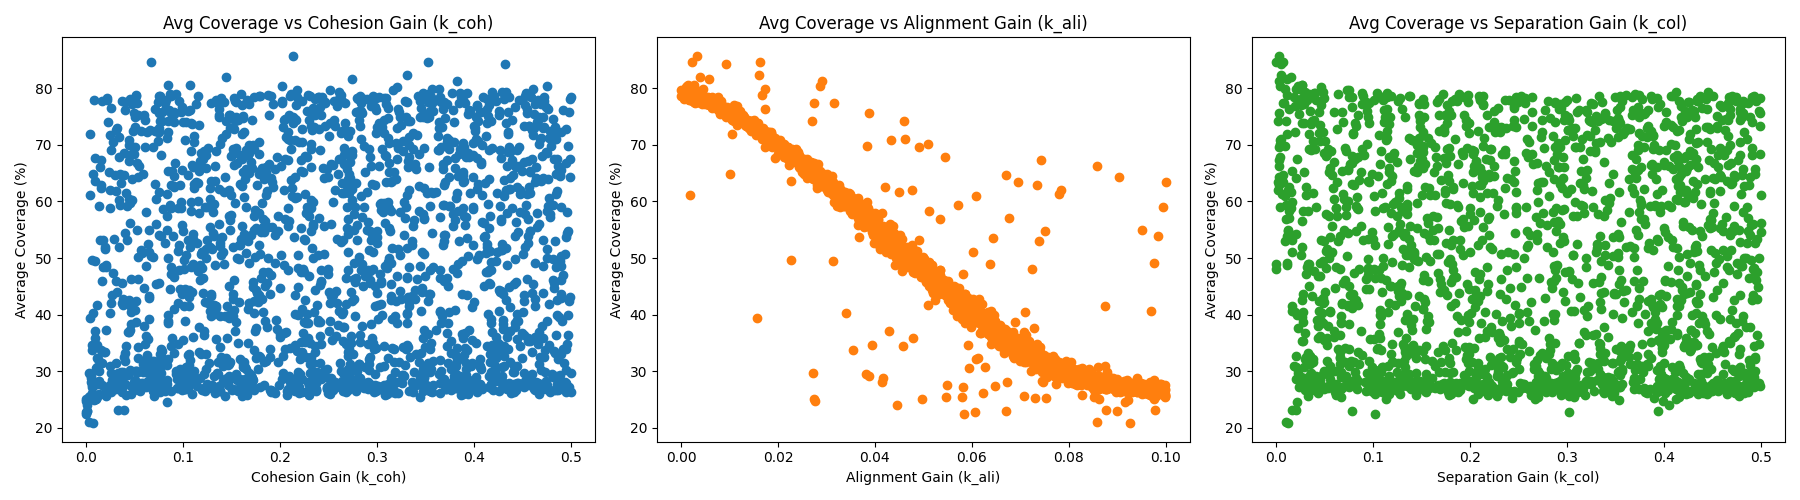
\includegraphics[width=\linewidth]{pics/cov_vs_gains/cafeteria_100.png}
\caption{Scatter plots showing coverage percentage for sampled behavioral gain values during parameter search in the Cafeteria environment, for \(N = 100\) boids. Each point represents the average coverage across three random seeds for a given configuration. Gain values correspond to (a) \(k_\text{coh}\), (b) \(k_\text{ali}\), and (c) \(k_\text{col}\). Coverage values are truncated to the nearest 0.1\%}
\label{fig:gains}
\end{figure}

\begin{figure}[h!]
    \centering
    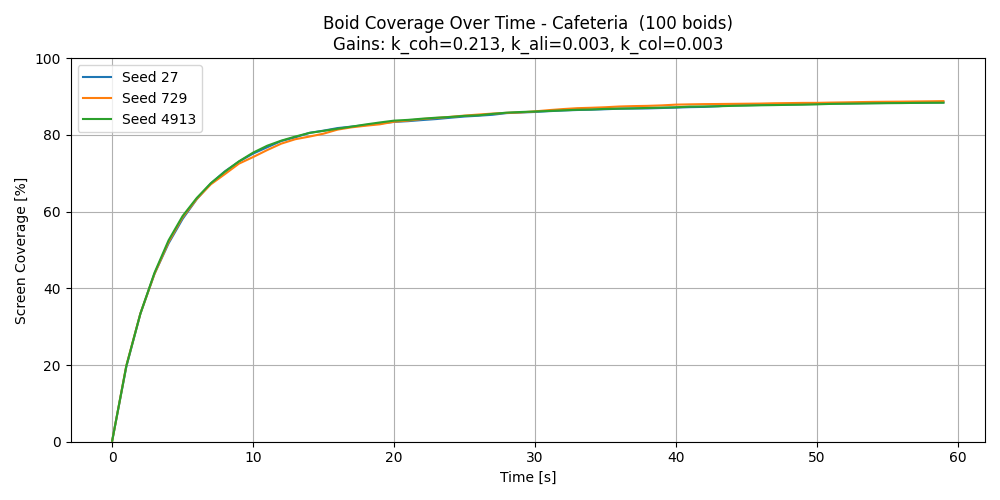
\includegraphics[width=0.7\linewidth]{optimal_cov_vs_time/cafeteria_100.png}
    \caption{Coverage over time for the best-performing gain vector \((k_\text{coh}, k_\text{ali}, k_\text{col}) = (0.213,0.003,0.003)\) in the Cafeteria environment for \(N = 100\) boids. Each line corresponds to a different random seed (27, 729, 4913).}
    \label{fig:caf_cov}
  \end{figure}

\begin{figure}[h!]
\centering
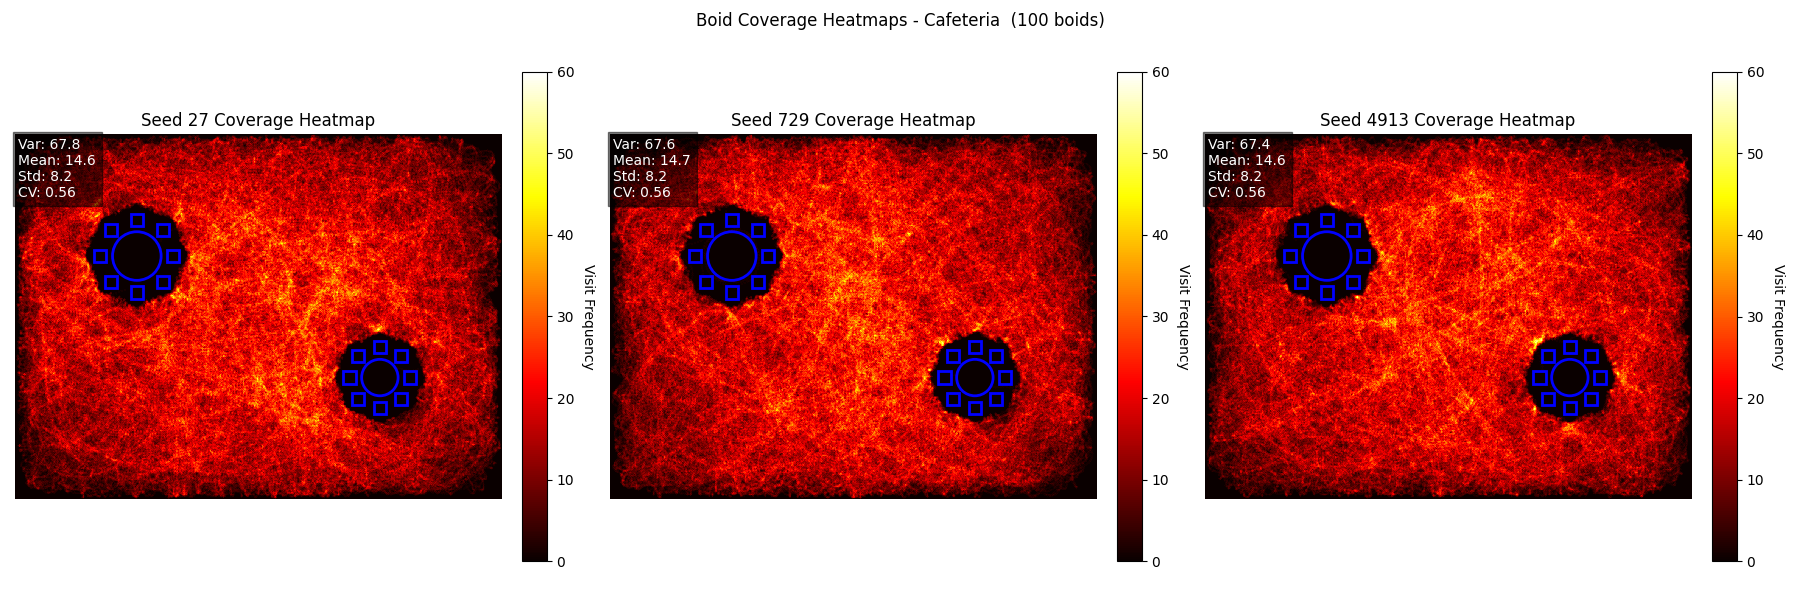
\includegraphics[width=\linewidth]{heatmaps/cafeteria_100.png}
\caption{Coverage heatmaps for the Cafeteria environment using the optimal gain vector across three random seeds (27, 729, 4913). Warmer colors indicate higher visitation frequency. Blue outlines represent obstacles, including circular tables and surrounding square chairs. Each image reflects the spatial distribution of cumulative agent movement over the 60-second simulation. Relevant statistical properties, such as coefficient of variation (CV) from the visitation frequencies, are also presented.}
\label{fig:caf_heatmap}
\end{figure}

\subsection{Coverage Uniformity}

While total coverage captures the extent of spatial exploration, it does not reflect how evenly agents distribute themselves. To address this, we computed the coefficient of variation (CV) from the heatmap visitation frequencies:
\begin{equation}\text{CV} = \frac{\sigma}{\mu}\end{equation}

where \(\mu\) and \(\sigma\) are the mean and standard deviation of visit counts across all traversable pixels. Lower CV values indicate more uniform exploration, while high CV suggests redundant trajectories or clustering. 

In open environments, such as the empty map, CV values remained consistently low (\(\approx\)0.45), reflecting highly uniform dispersion. In contrast, the Dense Cafeteria yielded CVs in the range of (0.92-1.07) for both swarm sizes, with 100 boids slightly outperforming 50 in terms of balance. The heatmaps reveal that while core regions were consistently visited, peripheral and occluded areas remained underexplored, especially in sparse swarms.

The Narrow Corridor further demonstrated the utility of CV. Even with similar total coverage, differences in how agents distributed themselves along the corridor led to CV fluctuations from 0.72 to 0.85. This shows that high coverage can still coincide with imbalanced spatial utilization, underscoring the importance of joint evaluation metrics. These results suggest that CV is a valuable metric in environments where spatial redundancy or clustering could degrade task efficiency.

\subsection{Environment-Specific Behavior and Effect of Boid Count}

The trends observed in the Cafeteria environment with 100 boids were broadly consistent across other maps, with key differences driven by obstacle density, spatial constraints, and swarm size. In the No Obstacles map, most gain configurations yielded near-maximal coverage. Exploration was rapid and consistent across seeds, with minimal sensitivity to cohesion or separation tuning. This suggests that, in open domains, simple repulsion and low alignment suffice to fully disperse the swarm.

Table~\ref{tab:coverage_by_seed_and_optimal_gain} reports per-seed coverage, average coverage, standard deviation, and the optimal gain configuration for each setting. The highest variance appears in the 50-boid trials within the Dense Cafeteria and Narrow Corridor environments, confirming the sensitivity of smaller swarms to initialization and local congestion. In contrast, the 100-boid configurations exhibited consistently higher coverage with lower variability.

\begin{table}[H]
    \footnotesize
    \centering
    \begin{tabular}{|l|c|c|c|c|c|c|c|}
    \hline
    \textbf{Environment} & \textbf{Boids} & \textbf{27} & \textbf{729} & \textbf{4913} & \textbf{Avg. Cov. [\%]} & \textbf{StdDev} & \textbf{Optimal Gains} \\
    \hline
    \multirow{2}{*}{Dense Cafeteria} 
        & 50  & 57.11 & 58.30 & 56.50 & 57.30 & 0.91 & (0.477, 0.017, 0.001) \\
        & 100 & 52.65 & 51.08 & 52.11 & 51.95 & 0.80 & (0.477, 0.017, 0.001) \\
    \hline
    \multirow{2}{*}{Cafeteria} 
        & 50  & 86.89 & 86.11 & 86.50 & 86.50 & 0.39 & (0.367, 0.024, 0.007) \\
        & 100 & 85.76 & 85.54 & 85.97 & 85.76 & 0.22 & (0.213, 0.003, 0.003) \\
    \hline
    \multirow{2}{*}{Narrow Corridor} 
        & 50  & 74.53 & 75.31 & 75.55 & 75.13 & 0.52 & (0.179, 0.044, 0.008) \\
        & 100 & 76.53 & 76.87 & 75.68 & 76.36 & 0.51 & (0.070, 0.010, 0.001) \\
    \hline
    \multirow{2}{*}{No Obstacles} 
        & 50  & 96.04 & 96.28 & 96.37 & 96.23 & 0.17 & (0.159, 0.003, 0.010) \\
        & 100 & 96.63 & 96.96 & 96.85 & 96.81 & 0.17 & (0.223, 0.001, 0.004) \\
    \hline
    \end{tabular}
    \caption{Per-seed and average coverage performance for each environment and swarm size, corresponding to the gain configuration that produced the highest average coverage. Standard deviations quantify variability across seeds. Gains are rounded to three decimal places.}
    \label{tab:coverage_by_seed_and_optimal_gain}
\end{table}

To further analyze spatial consistency, Table~\ref{tab:normalized_cv} presents the normalized coefficient of variation (CV) in heatmap visitation frequencies for each seed and environment. Higher CV values indicate more uneven exploration. As expected, environments with more obstacles—especially the Dense Cafeteria—exhibited higher CVs, particularly with 50 boids. In contrast, coverage in the Empty map was both complete and spatially uniform, with CV values below 0.46 in all trials.

\begin{table}[H]
    \footnotesize
    \centering
    \begin{tabular}{|l|c|c|c|c|c|}
    \hline
    \textbf{Environment} & \textbf{Boids} & \textbf{27} & \textbf{729} & \textbf{4913} & \textbf{Avg. Norm. CV} \\
    \hline
    \multirow{2}{*}{Dense Cafeteria}    
        & 50  & 1.0685 & 0.9495 & 1.0126 & 1.0102 \\
        & 100 & 1.0399 & 0.9760 & 0.9187 & 0.9782 \\
    \hline
    \multirow{2}{*}{Cafeteria}          
        & 50  & 0.6312 & 0.6424 & 0.6457 & 0.6398 \\
        & 100 & 0.5634 & 0.5584 & 0.5608 & 0.5609 \\
    \hline
    \multirow{2}{*}{Narrow Corridor}    
        & 50  & 0.7358 & 0.7886 & 0.7211 & 0.7485 \\
        & 100 & 0.8462 & 0.8026 & 0.8045 & 0.8178 \\
    \hline
    \multirow{2}{*}{No Obstacles}       
        & 50  & 0.4526 & 0.4519 & 0.4581 & 0.4542 \\
        & 100 & 0.4409 & 0.4467 & 0.4447 & 0.4441 \\
    \hline
    \end{tabular}
    \caption{Normalized coefficient of variation (CV) in heatmap visitation frequency for each environment and swarm size, evaluated using the optimal gain vector. Values are reported per seed and averaged across seeds. Lower CV indicates more uniform spatial coverage.}
    \label{tab:normalized_cv}
\end{table}

These results highlight that increasing the swarm size from 50 to 100 improved both overall coverage and spatial uniformity across all environments. The benefits were especially pronounced in cluttered maps, where higher agent density helped reduce fragmentation and improved robustness to initialization. In the Narrow Corridor, for instance, low boid counts often resulted in incomplete coverage due to agents failing to propagate beyond the bottleneck.

The remaining coverage heatmaps and cumulative coverage plots for all environments and swarm sizes are available at the following link:
\url{https://github.com/destrospooder/boids/tree/main/report/pics}. They can also be found in Appendix A.

\subsection{Limitations and Future Work}

While the simulation demonstrates that tuning boid parameters can enhance exploration performance, several assumptions constrain the applicability of these results to real-world robotic systems. First, the model assumes perfect sensing. Each agent is assumed to have accurate and instantaneous access to the states of all neighbors within its perception radius and field of view. This ignores sensor noise, occlusion, and communication delays, all of which can significantly impact behavior in physical deployments. Future work should explore how degraded sensing or limited bandwidth affects coordination and coverage.

Second, the agents are homogeneous. All boids use the same gain values, perception parameters, and motion constraints. While this simplifies analysis, it neglects the possibility of introducing agent heterogeneity to improve robustness or task efficiency. Exploring the effect of diverse behavior profiles, or allowing agents to adapt gains based on local context, may yield more resilient policies.

Third, the environments are static and fully known. Obstacles are placed at initialization and remain fixed for the duration of the simulation. In practical exploration scenarios, agents must often navigate partially known or dynamic environments. Incorporating real-time mapping, obstacle detection, and local replanning would increase the relevance of the model for deployed systems.

Fourth, the optimization objective is limited to total coverage. While coverage uniformity is evaluated using the coefficient of variation, it is not used to guide the parameter search directly. Incorporating a joint objective that balances extent and uniformity could produce more efficient and evenly distributed behaviors, especially in cluttered maps.

Fifth, the simulation omits physical dynamics such as inertia, acceleration limits beyond a scalar cap, and energy consumption. These factors are important in domains like aerial or underwater robotics, where control authority is limited and motion is governed by more complex dynamics. Additionally, the current wall repulsion gain is set relatively high (10) to enforce strict boundary compliance in the absence of physical barriers or damping. While this is effective for containment in simulation, it may lead to unrealistic behaviors or unstable oscillations near walls if transferred directly to physical systems. Incorporating smoother wall interactions or physically plausible damping models could improve realism.

Finally, the gain space was explored via random search, which, while robust and embarrassingly parallel, is inefficient in high-dimensional or multi-objective contexts. While sufficient for coarse exploration, this method becomes inefficient as the parameter space grows or if multiple objectives are introduced. More structured search methods, such as gradient-free optimizers or model-based approaches, could accelerate convergence and better exploit the structure of the gain-performance landscape.

\section{Conclusion}

This study demonstrates that the boids model, when tuned appropriately, can serve as a viable decentralized framework for distributed coverage tasks in complex environments. By systematically optimizing the core behavioral parameters governing alignment, cohesion, and separation, significant improvements in exploration efficiency were achieved, particularly in cluttered scenarios where coordination must be balanced with dispersion. The results suggest that minimal alignment and arbitrary levels of cohesion and separation, yields the most effective coverage behavior under spatial constraints. These insights support the broader applicability of bio-inspired swarm algorithms in real-world robotic systems, particularly in scenarios where scalability, robustness, and adaptability are critical.

The complete dataset, simulator, optimization, and postprocessing scripts are available at \url{https://github.com/destrospooder/boids}.

\bibliography{references}

\newpage

\appendix
\section{Additional Coverage Figures}

%----------------------------------------------------------------
% Cafeteria, N = 50
\begin{figure}[h!]
  \centering
  \begin{subfigure}[b]{0.32\linewidth}
    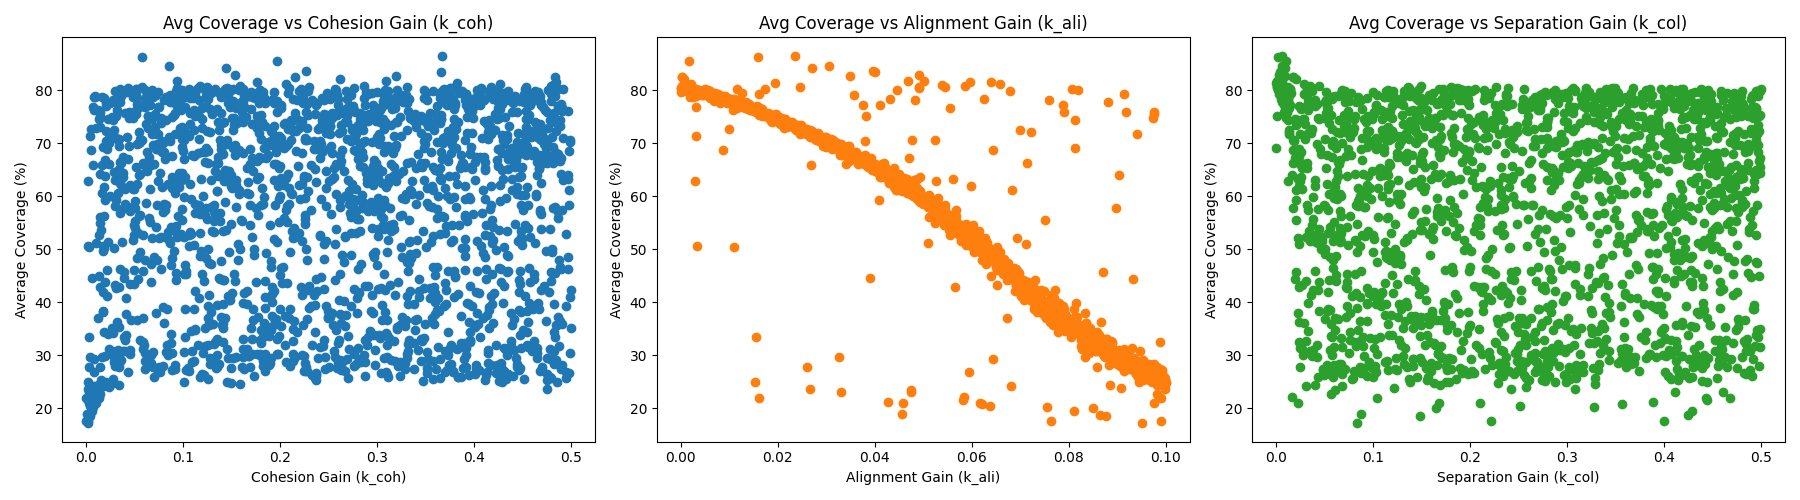
\includegraphics[width=\linewidth]{cov_vs_gains/cafeteria_50.png}
    \caption{Coverage vs.~gains for the Cafeteria map with $N=50$ boids.}
    \label{fig:app:caf50_gains}
  \end{subfigure}\hfill
  \begin{subfigure}[b]{0.32\linewidth}
    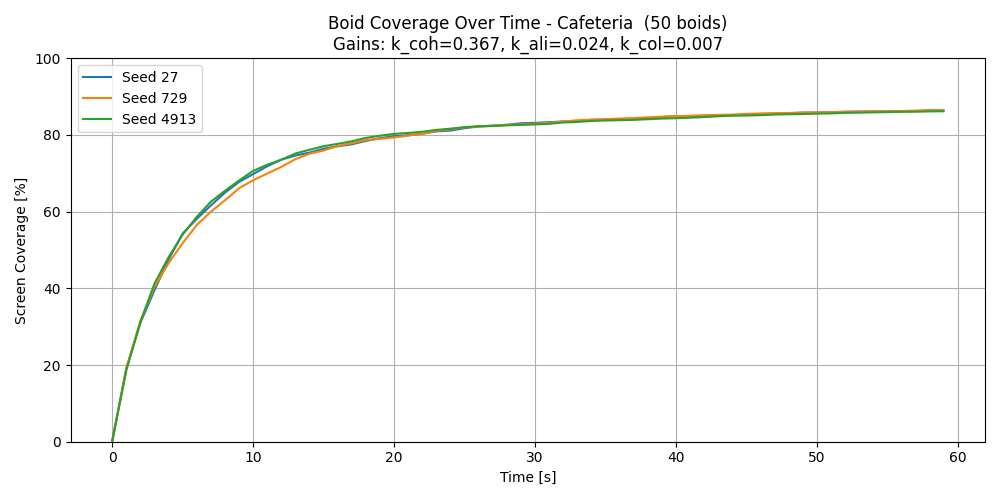
\includegraphics[width=\linewidth]{optimal_cov_vs_time/cafeteria_50.png}
    \caption{Coverage over time for the Cafeteria map with $N=50$ boids.}
    \label{fig:app:caf50_time}
  \end{subfigure}\hfill
  \begin{subfigure}[b]{0.32\linewidth}
    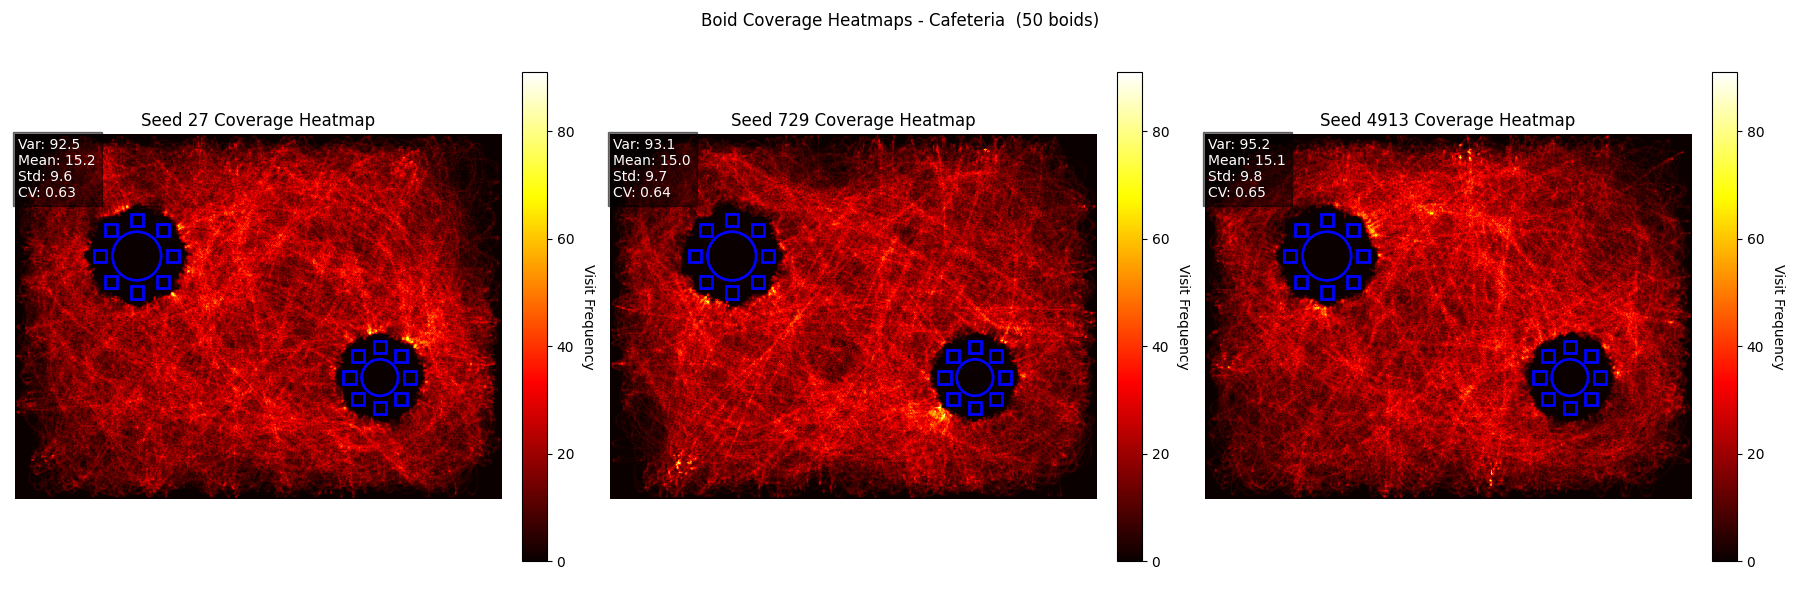
\includegraphics[width=\linewidth]{heatmaps/cafeteria_50.png}
    \caption{Coverage heatmap for the Cafeteria map with $N=50$ boids.}
    \label{fig:app:caf50_heat}
  \end{subfigure}
  \caption{Coverage analysis for the Cafeteria environment with $N=50$ boids: (a) relationship between behavioral gains and coverage, (b) cumulative coverage over time, (c) visitation frequency heatmap.}
  \label{fig:app:cafeteria50}
\end{figure}

%----------------------------------------------------------------
% Dense Cafeteria, N = 50
\begin{figure}[h!]
  \centering
  \begin{subfigure}[b]{0.32\linewidth}
    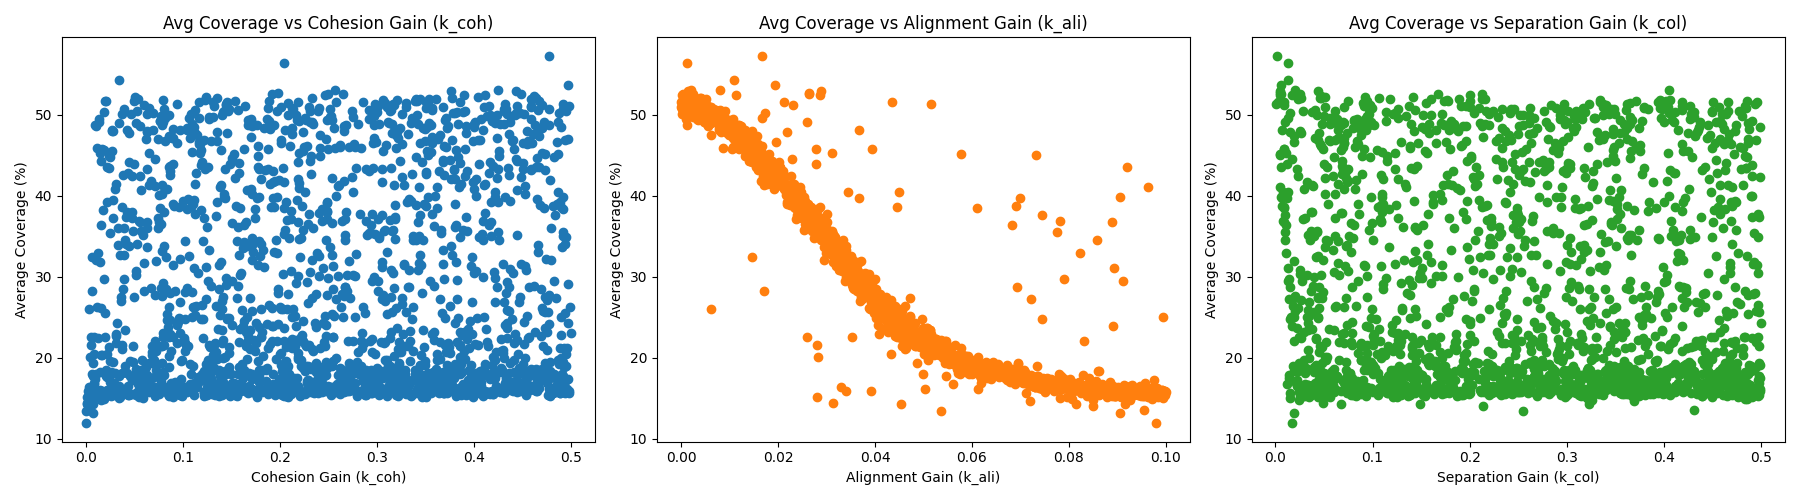
\includegraphics[width=\linewidth]{cov_vs_gains/dense_50.png}
    \caption{Coverage vs.~gains for the Dense Cafeteria map with $N=50$ boids.}
    \label{fig:app:dense50_gains}
  \end{subfigure}\hfill
  \begin{subfigure}[b]{0.32\linewidth}
    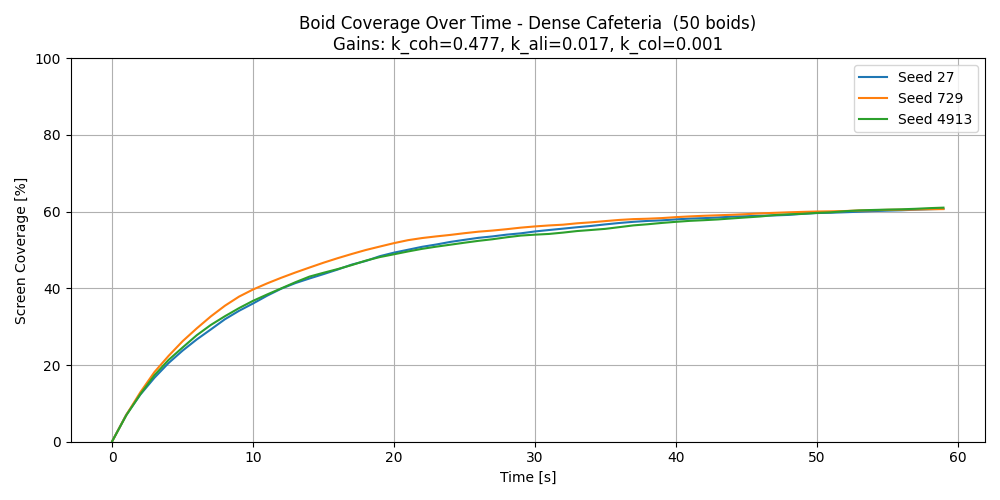
\includegraphics[width=\linewidth]{optimal_cov_vs_time/dense_50.png}
    \caption{Coverage over time for the Dense Cafeteria map with $N=50$ boids.}
    \label{fig:app:dense50_time}
  \end{subfigure}\hfill
  \begin{subfigure}[b]{0.32\linewidth}
    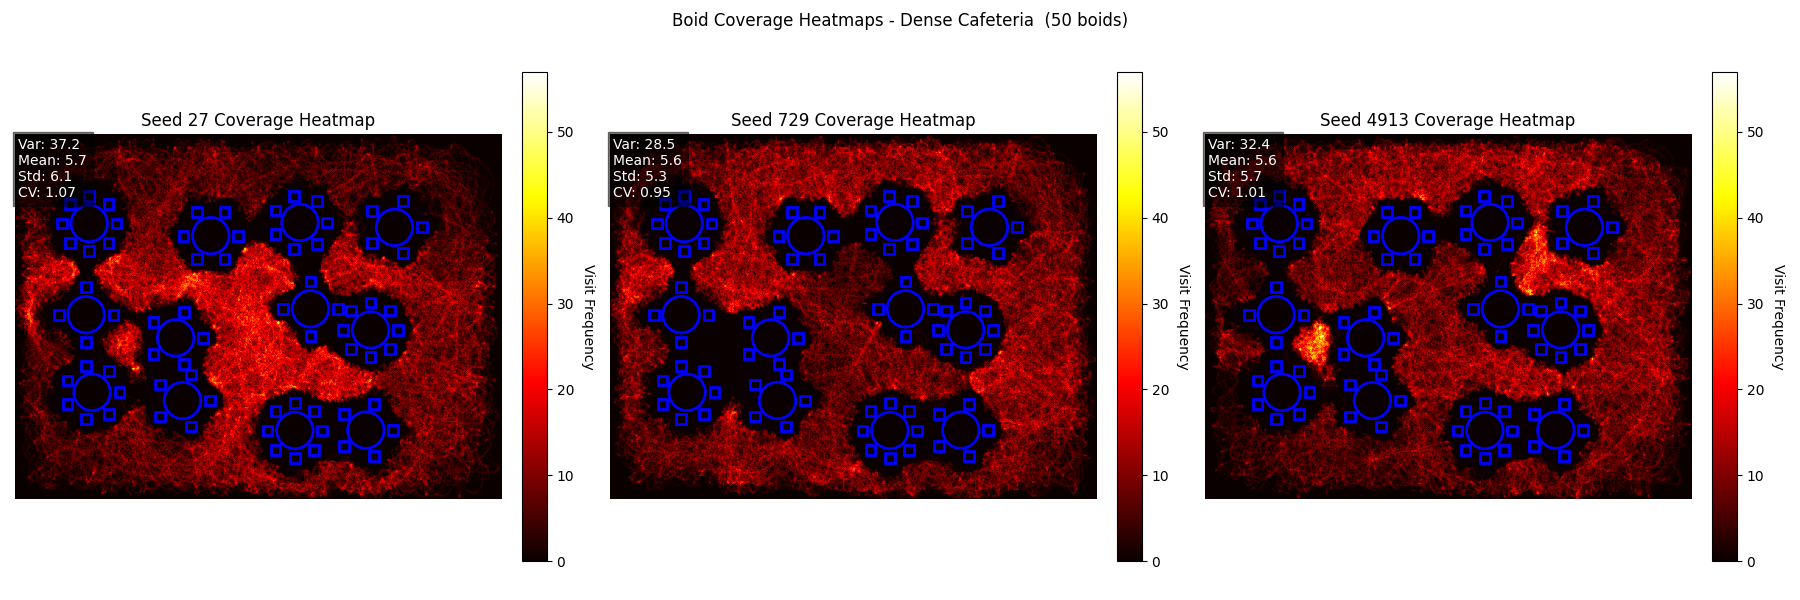
\includegraphics[width=\linewidth]{heatmaps/dense_50.png}
    \caption{Coverage heatmap for the Dense Cafeteria map with $N=50$ boids.}
    \label{fig:app:dense50_heat}
  \end{subfigure}
  \caption{Coverage analysis for the Dense Cafeteria environment with $N=50$ boids: (a) coverage vs.~gains, (b) cumulative coverage over time, (c) coverage heatmap.}
  \label{fig:app:densecaf50}
\end{figure}

%----------------------------------------------------------------
% Dense Cafeteria, N = 100
\begin{figure}[h!]
  \centering
  \begin{subfigure}[b]{0.32\linewidth}
    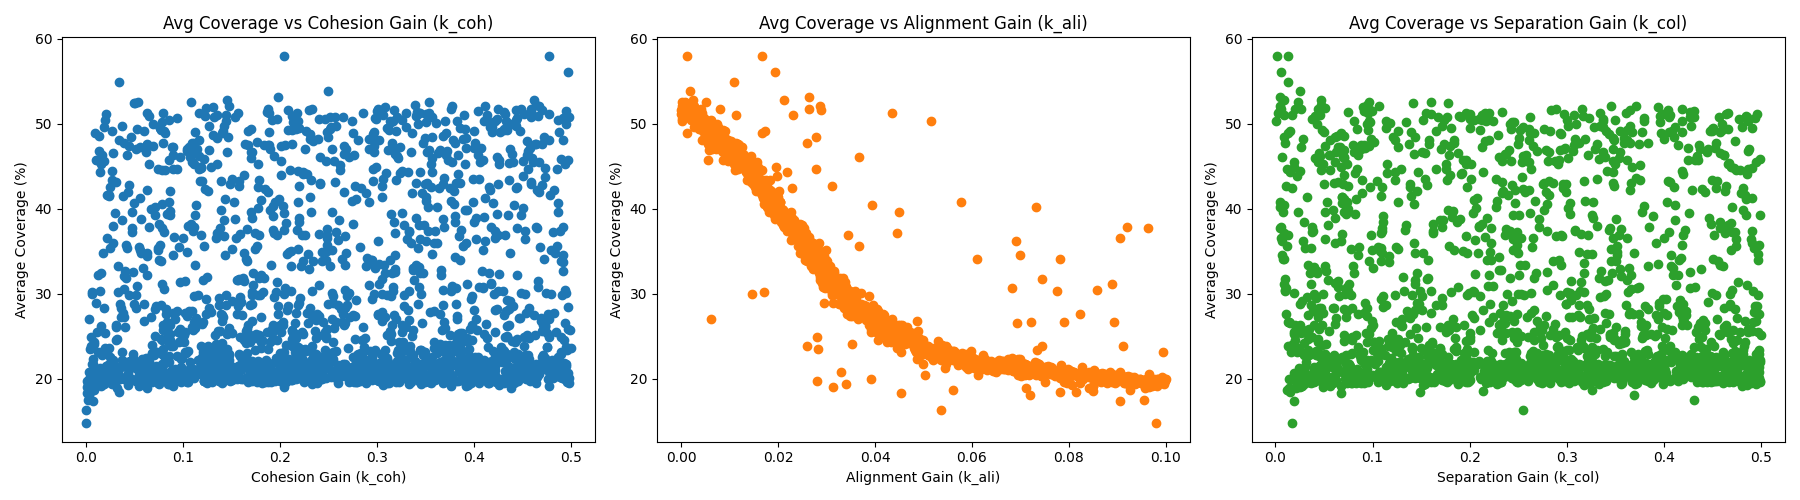
\includegraphics[width=\linewidth]{cov_vs_gains/dense_100.png}
    \caption{Coverage vs.~gains for the Dense Cafeteria map with $N=100$ boids.}
    \label{fig:app:dense100_gains}
  \end{subfigure}\hfill
  \begin{subfigure}[b]{0.32\linewidth}
    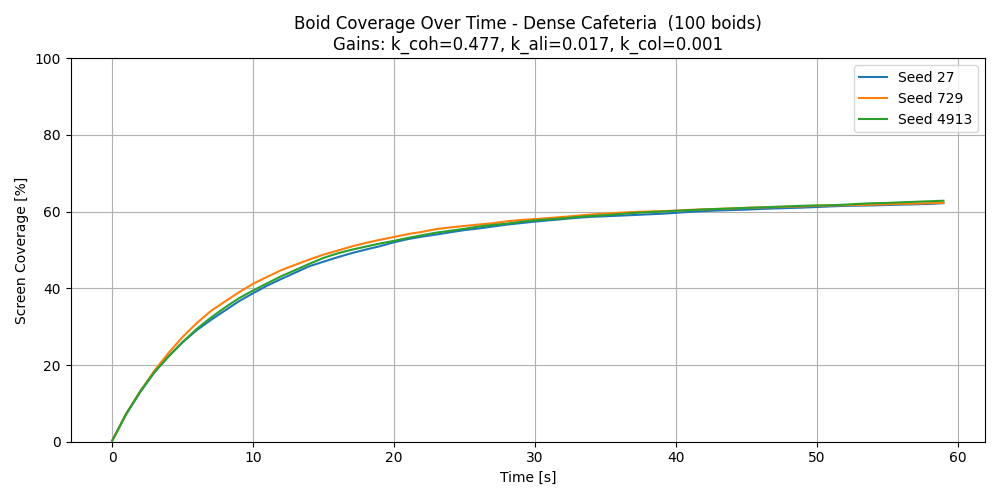
\includegraphics[width=\linewidth]{optimal_cov_vs_time/dense_100.png}
    \caption{Coverage over time for the Dense Cafeteria map with $N=100$ boids.}
    \label{fig:app:dense100_time}
  \end{subfigure}\hfill
  \begin{subfigure}[b]{0.32\linewidth}
    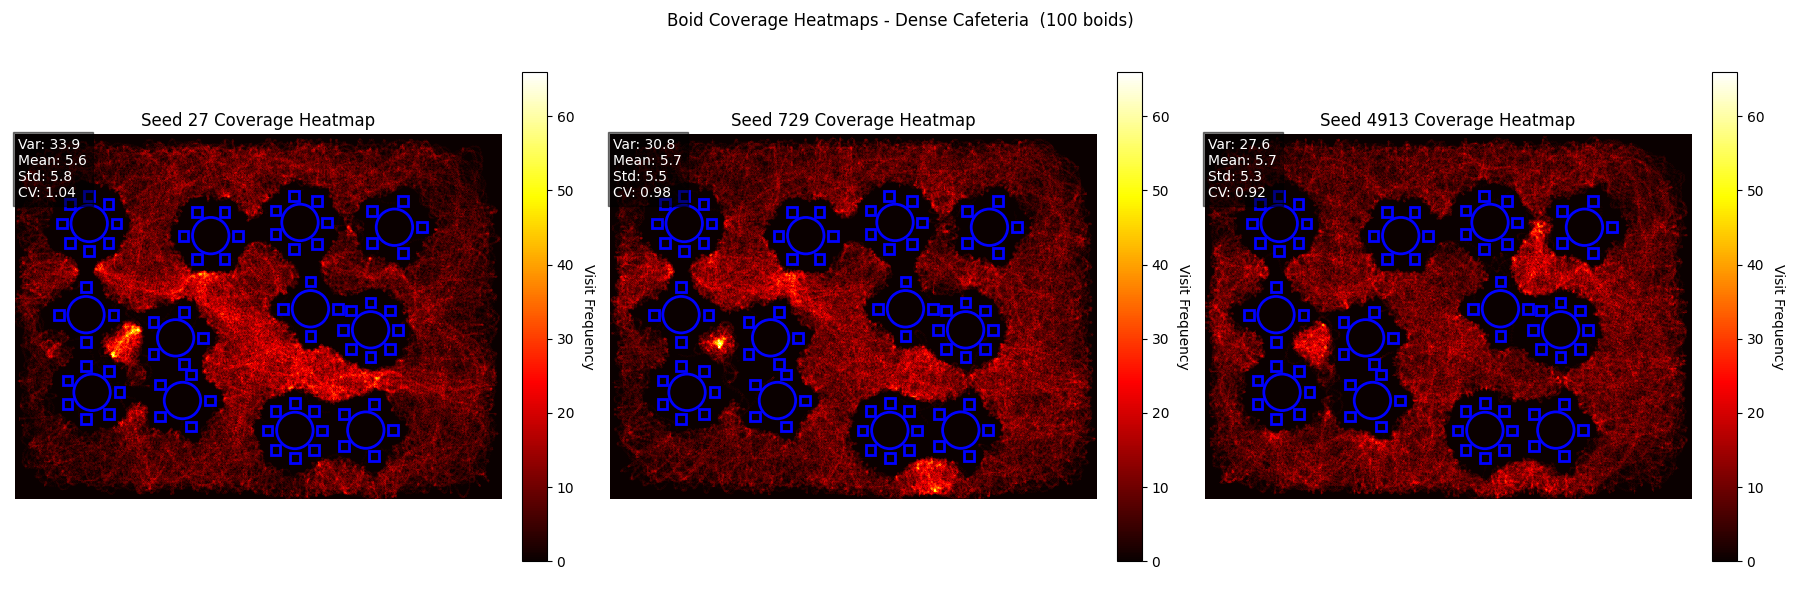
\includegraphics[width=\linewidth]{heatmaps/dense_100.png}
    \caption{Coverage heatmap for the Dense Cafeteria map with $N=100$ boids.}
    \label{fig:app:dense100_heat}
  \end{subfigure}
  \caption{Coverage analysis for the Dense Cafeteria environment with $N=100$ boids: (a) coverage vs.~gains, (b) cumulative coverage over time, (c) coverage heatmap.}
  \label{fig:app:densecaf100}
\end{figure}

%----------------------------------------------------------------
% Empty Map, N = 50
\begin{figure}[h!]
  \centering
  \begin{subfigure}[b]{0.32\linewidth}
    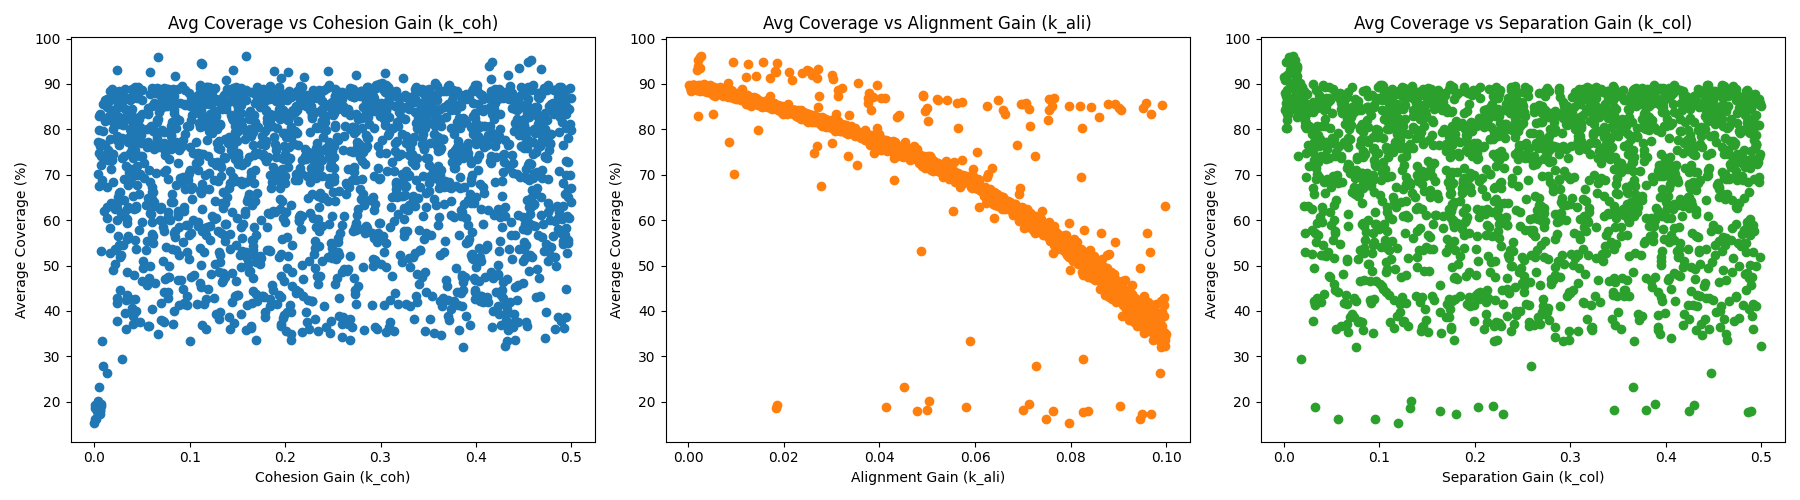
\includegraphics[width=\linewidth]{cov_vs_gains/empty_50.png}
    \caption{Coverage vs.~gains for the Empty map with $N=50$ boids.}
    \label{fig:app:empty50_gains}
  \end{subfigure}\hfill
  \begin{subfigure}[b]{0.32\linewidth}
    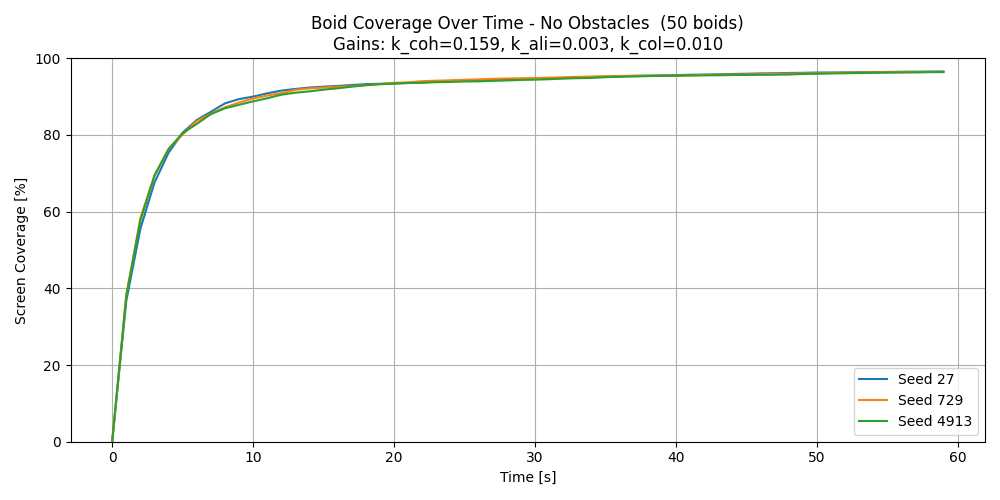
\includegraphics[width=\linewidth]{optimal_cov_vs_time/empty_50.png}
    \caption{Coverage over time for the Empty map with $N=50$ boids.}
    \label{fig:app:empty50_time}
  \end{subfigure}\hfill
  \begin{subfigure}[b]{0.32\linewidth}
    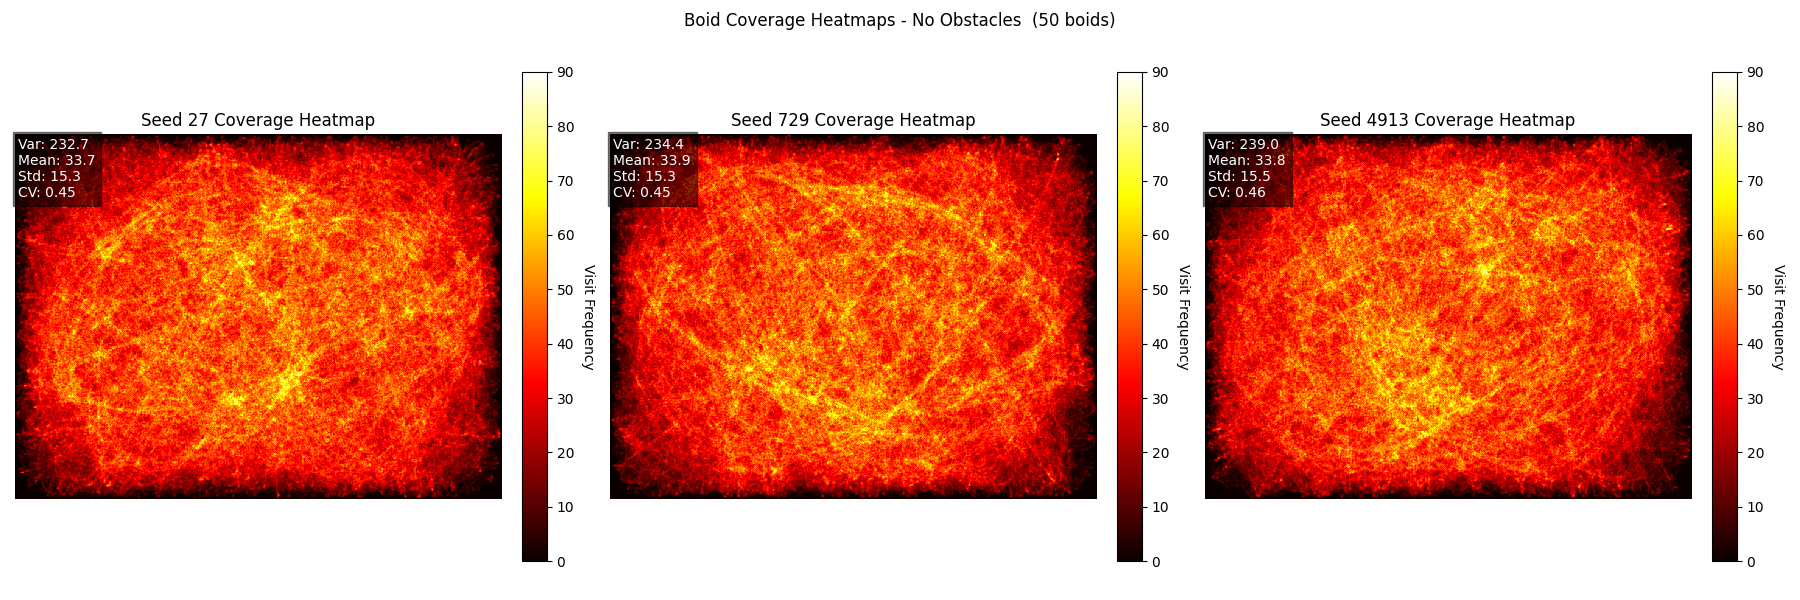
\includegraphics[width=\linewidth]{heatmaps/empty_50.png}
    \caption{Coverage heatmap for the Empty map with $N=50$ boids.}
    \label{fig:app:empty50_heat}
  \end{subfigure}
  \caption{Coverage analysis for the Empty environment with $N=50$ boids: (a) coverage vs.~gains, (b) cumulative coverage over time, (c) coverage heatmap.}
  \label{fig:app:empty50}
\end{figure}

%----------------------------------------------------------------
% Empty Map, N = 100
\begin{figure}[h!]
  \centering
  \begin{subfigure}[b]{0.32\linewidth}
    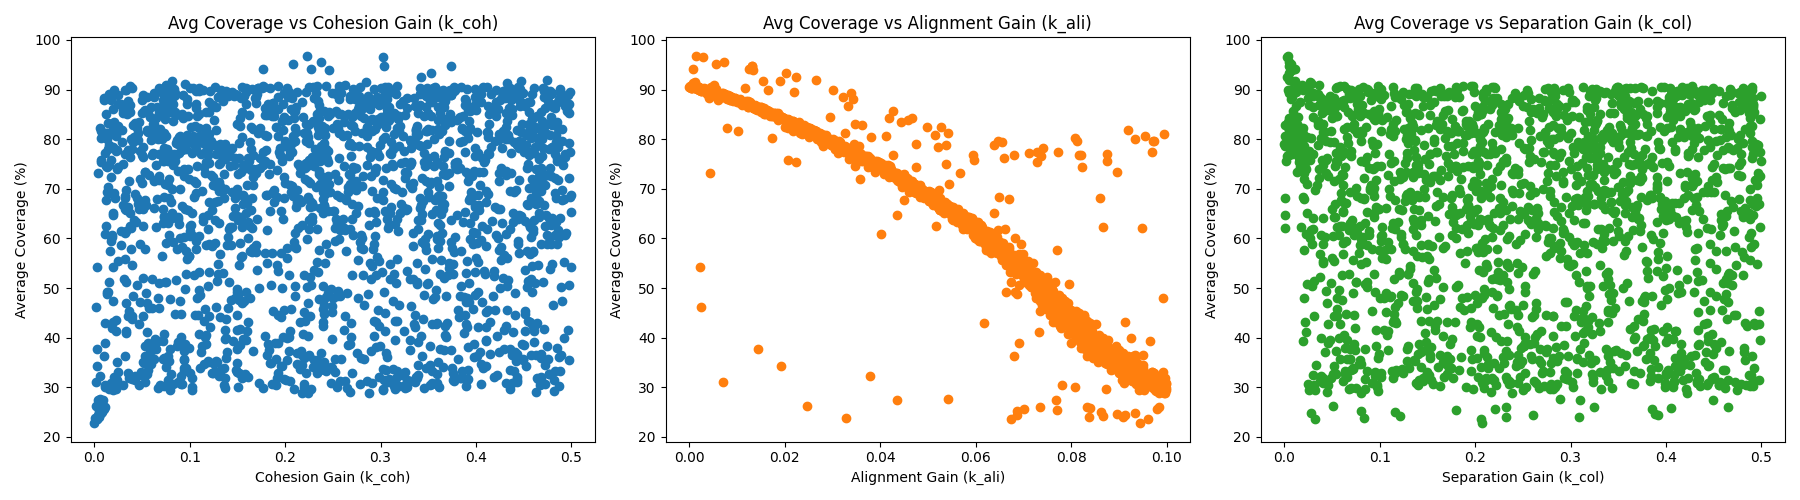
\includegraphics[width=\linewidth]{cov_vs_gains/empty_100.png}
    \caption{Coverage vs.~gains for the Empty map with $N=100$ boids.}
    \label{fig:app:empty100_gains}
  \end{subfigure}\hfill
  \begin{subfigure}[b]{0.32\linewidth}
    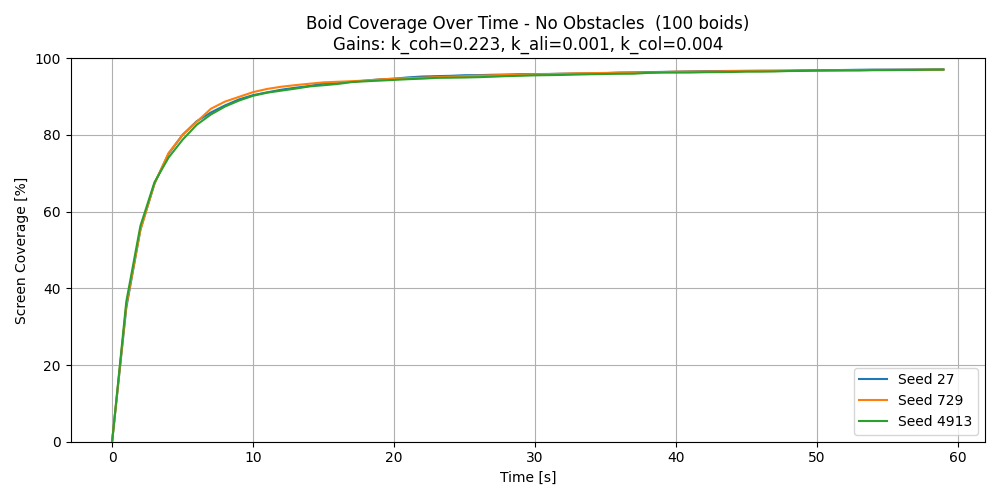
\includegraphics[width=\linewidth]{optimal_cov_vs_time/empty_100.png}
    \caption{Coverage over time for the Empty map with $N=100$ boids.}
    \label{fig:app:empty100_time}
  \end{subfigure}\hfill
  \begin{subfigure}[b]{0.32\linewidth}
    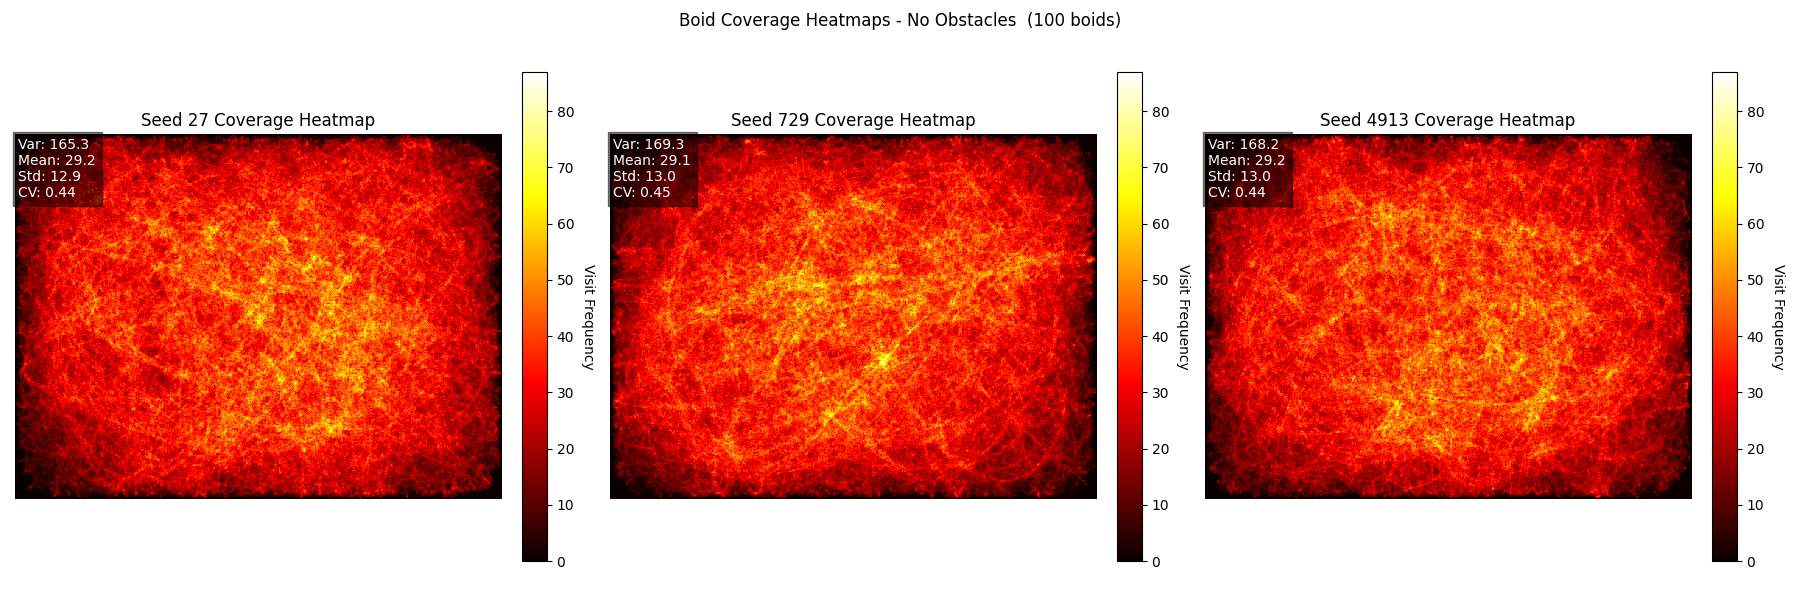
\includegraphics[width=\linewidth]{heatmaps/empty_100.png}
    \caption{Coverage heatmap for the Empty map with $N=100$ boids.}
    \label{fig:app:empty100_heat}
  \end{subfigure}
  \caption{Coverage analysis for the Empty environment with $N=100$ boids: (a) coverage vs.~gains, (b) cumulative coverage over time, (c) coverage heatmap.}
  \label{fig:app:empty100}
\end{figure}

%----------------------------------------------------------------
% Narrow Corridor, N = 50
\begin{figure}[h!]
  \centering
  \begin{subfigure}[b]{0.32\linewidth}
    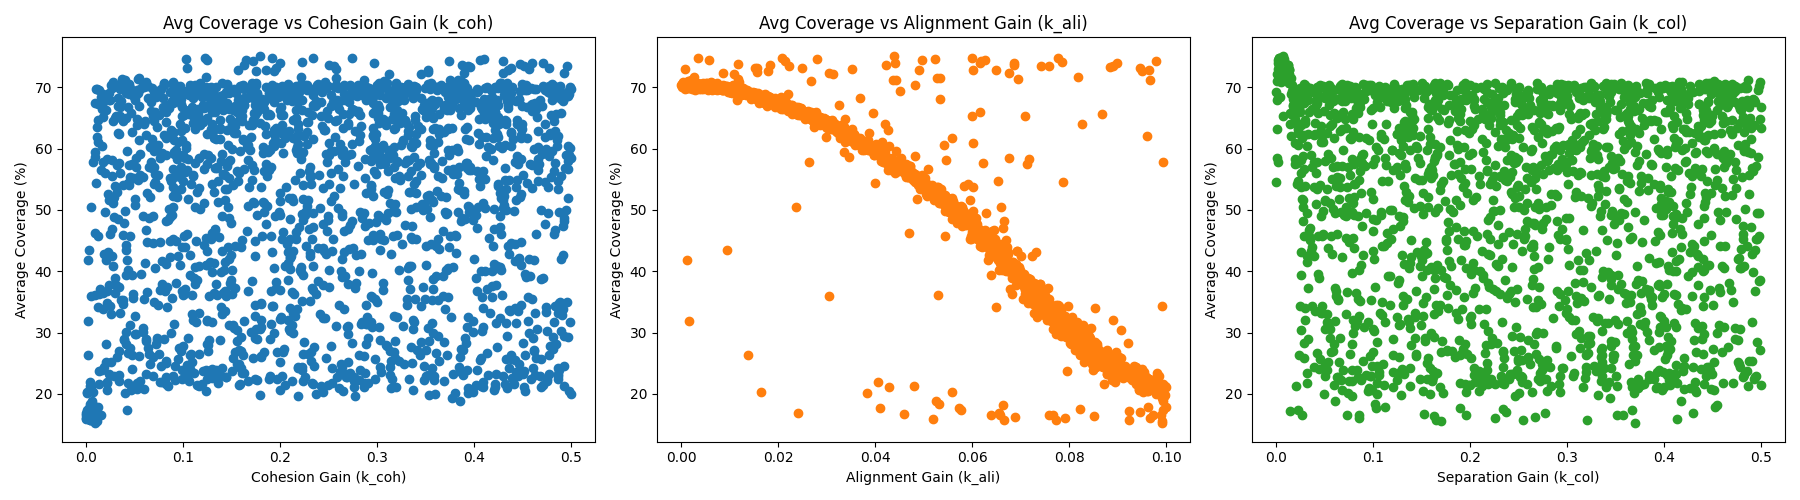
\includegraphics[width=\linewidth]{cov_vs_gains/narrow_50.png}
    \caption{Coverage vs.~gains for the Narrow Corridor map with $N=50$ boids.}
    \label{fig:app:narrow50_gains}
  \end{subfigure}\hfill
  \begin{subfigure}[b]{0.32\linewidth}
    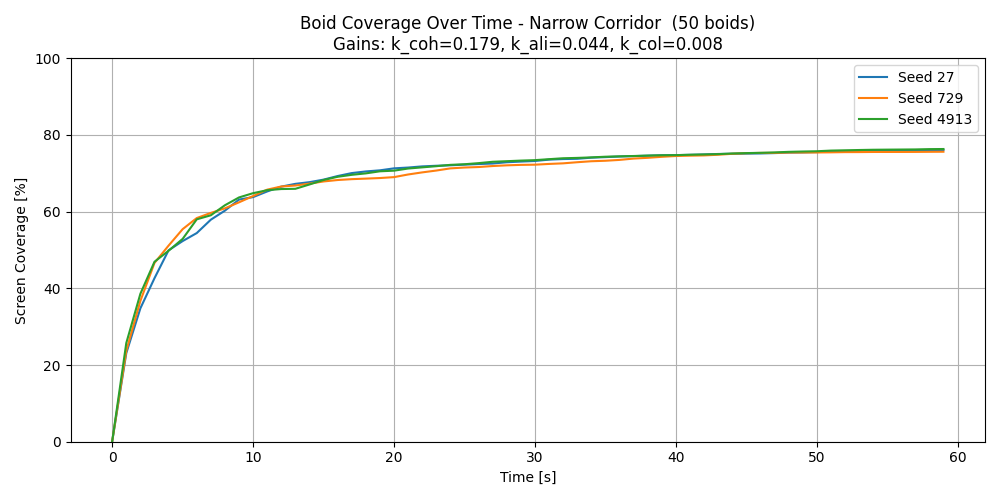
\includegraphics[width=\linewidth]{optimal_cov_vs_time/narrow_50.png}
    \caption{Coverage over time for the Narrow Corridor map with $N=50$ boids.}
    \label{fig:app:narrow50_time}
  \end{subfigure}\hfill
  \begin{subfigure}[b]{0.32\linewidth}
    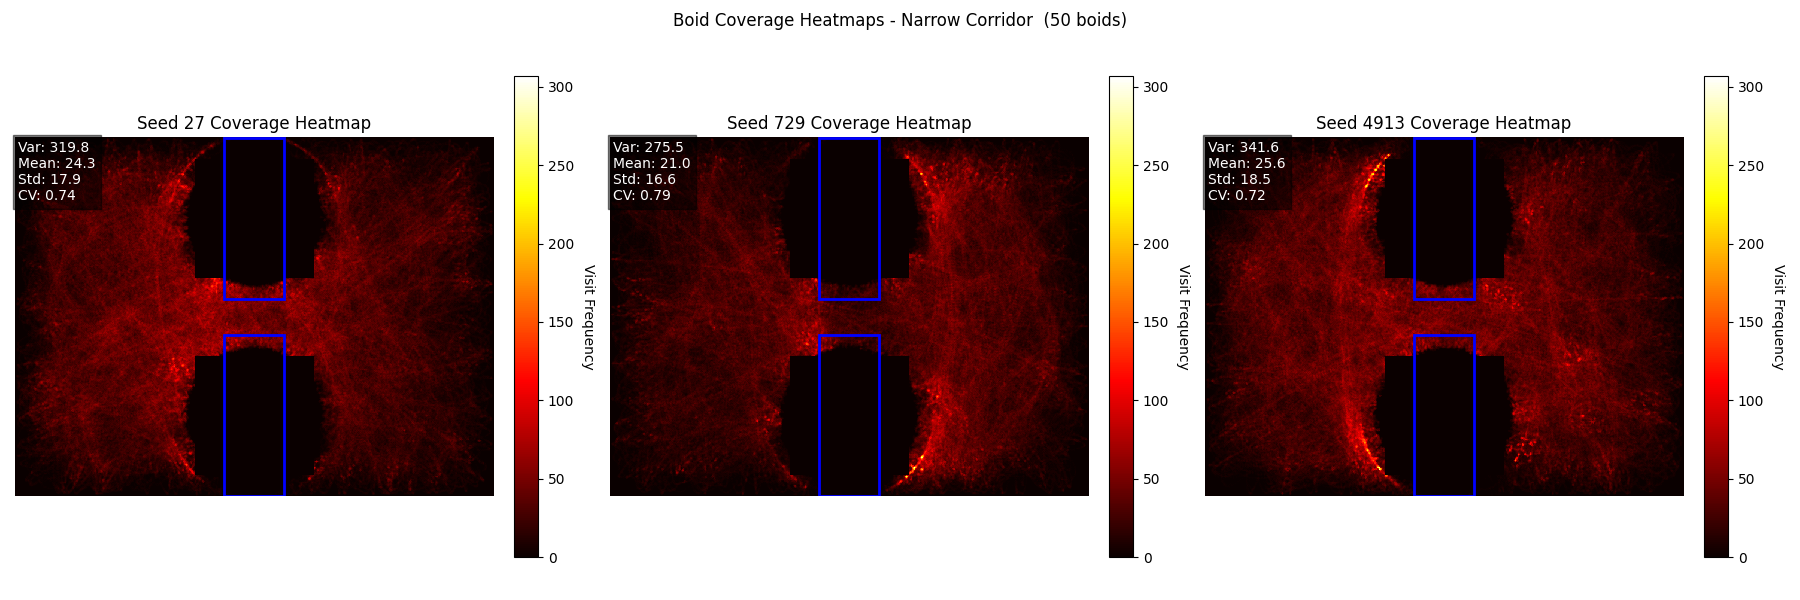
\includegraphics[width=\linewidth]{heatmaps/narrow_50.png}
    \caption{Coverage heatmap for the Narrow Corridor map with $N=50$ boids.}
    \label{fig:app:narrow50_heat}
  \end{subfigure}
  \caption{Coverage analysis for the Narrow Corridor environment with $N=50$ boids: (a) coverage vs.~gains, (b) cumulative coverage over time, (c) coverage heatmap.}
  \label{fig:app:narrow50}
\end{figure}

%----------------------------------------------------------------
% Narrow Corridor, N = 100
\begin{figure}[h!]
  \centering
  \begin{subfigure}[b]{0.32\linewidth}
    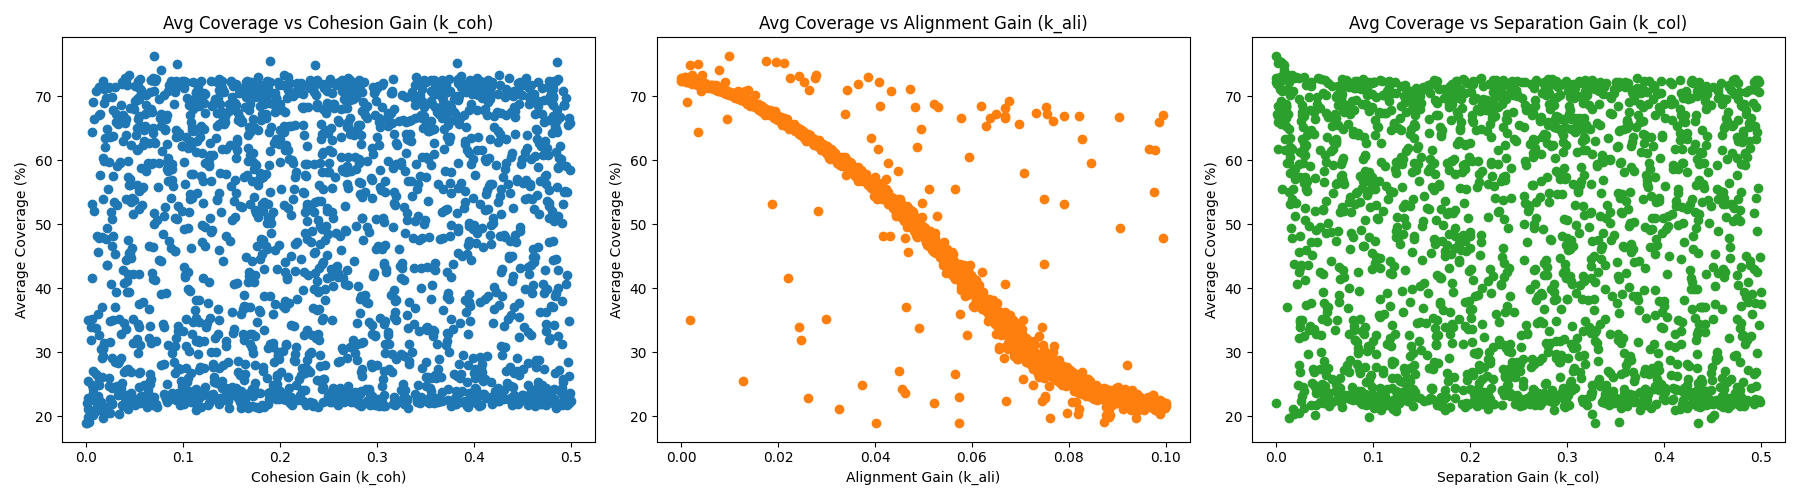
\includegraphics[width=\linewidth]{cov_vs_gains/narrow_100.png}
    \caption{Coverage vs.~gains for the Narrow Corridor map with $N=100$ boids.}
    \label{fig:app:narrow100_gains}
  \end{subfigure}\hfill
  \begin{subfigure}[b]{0.32\linewidth}
    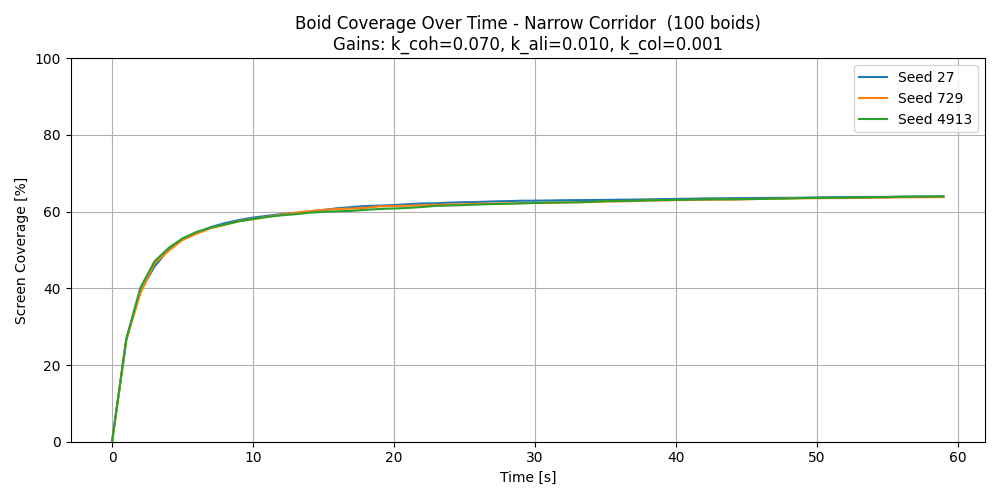
\includegraphics[width=\linewidth]{optimal_cov_vs_time/narrow_100.png}
    \caption{Coverage over time for the Narrow Corridor map with $N=100$ boids.}
    \label{fig:app:narrow100_time}
  \end{subfigure}\hfill
  \begin{subfigure}[b]{0.32\linewidth}
    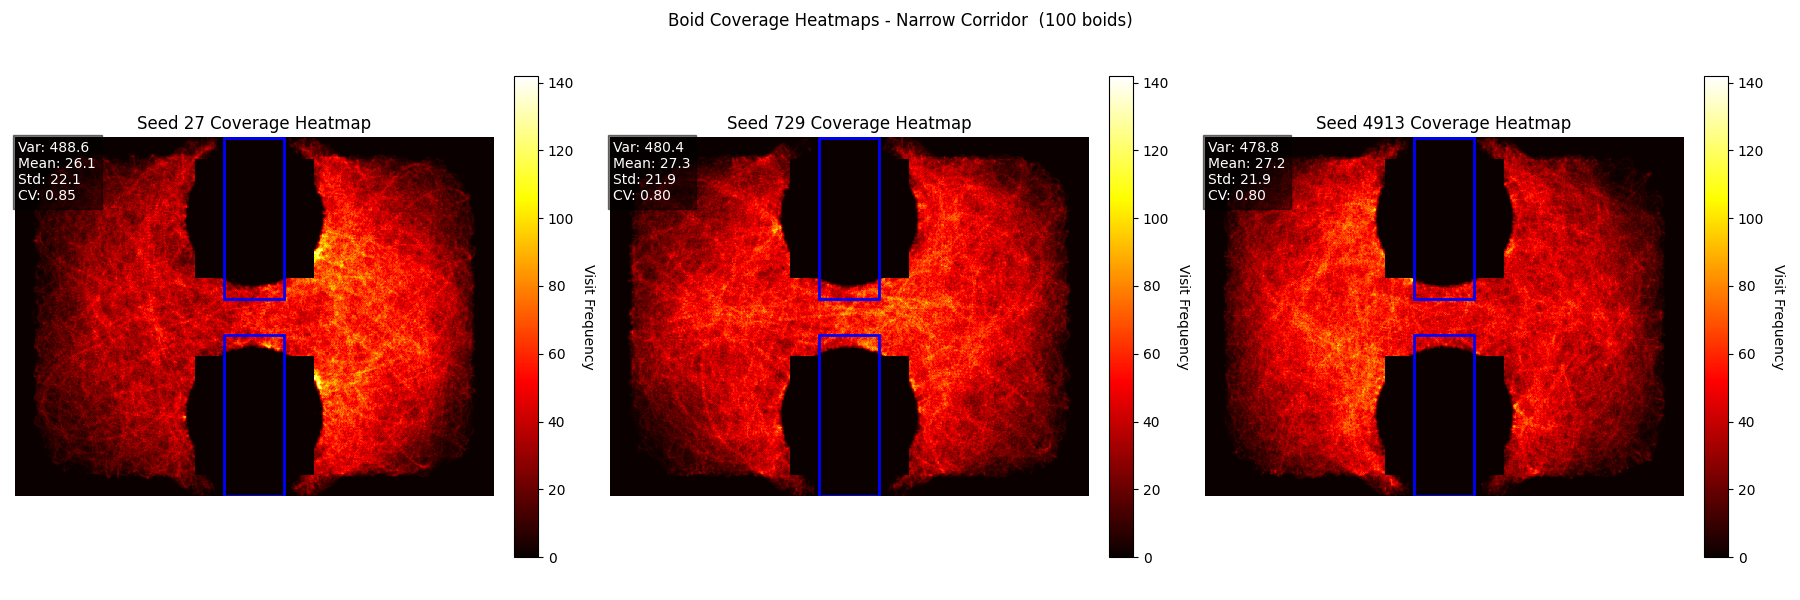
\includegraphics[width=\linewidth]{heatmaps/narrow_100.png}
    \caption{Coverage heatmap for the Narrow Corridor map with $N=100$ boids.}
    \label{fig:app:narrow100_heat}
  \end{subfigure}
  \caption{Coverage analysis for the Narrow Corridor environment with $N=100$ boids: (a) coverage vs.~gains, (b) cumulative coverage over time, (c) coverage heatmap.}
  \label{fig:app:narrow100}
\end{figure}


\appendix
\section{Additional Figures}

%----------------------------------------------------------------
% Cafeteria, N = 50
\begin{figure}[h!]
  \centering
  \begin{subfigure}[b]{0.32\linewidth}
    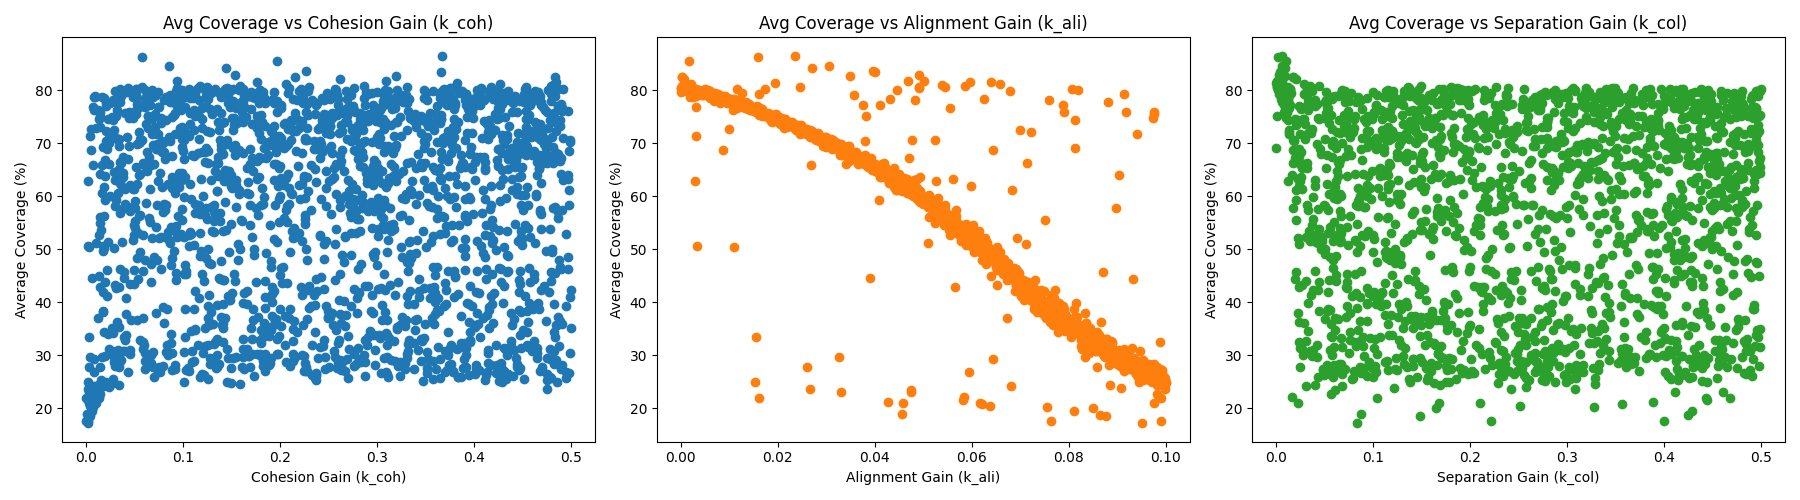
\includegraphics[width=\linewidth]{cov_vs_gains/cafeteria_50.png}
    \caption{Coverage vs.~gains for the Cafeteria map with $N=50$ boids.}
    \label{fig:app:caf50_gains}
  \end{subfigure}\hfill
  \begin{subfigure}[b]{0.32\linewidth}
    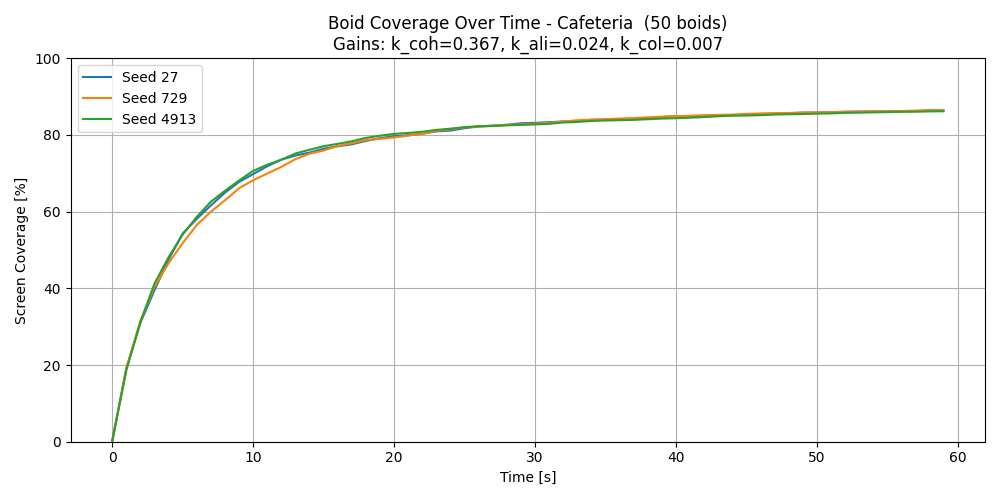
\includegraphics[width=\linewidth]{optimal_cov_vs_time/cafeteria_50.png}
    \caption{Coverage over time for the Cafeteria map with $N=50$ boids.}
    \label{fig:app:caf50_time}
  \end{subfigure}\hfill
  \begin{subfigure}[b]{0.32\linewidth}
    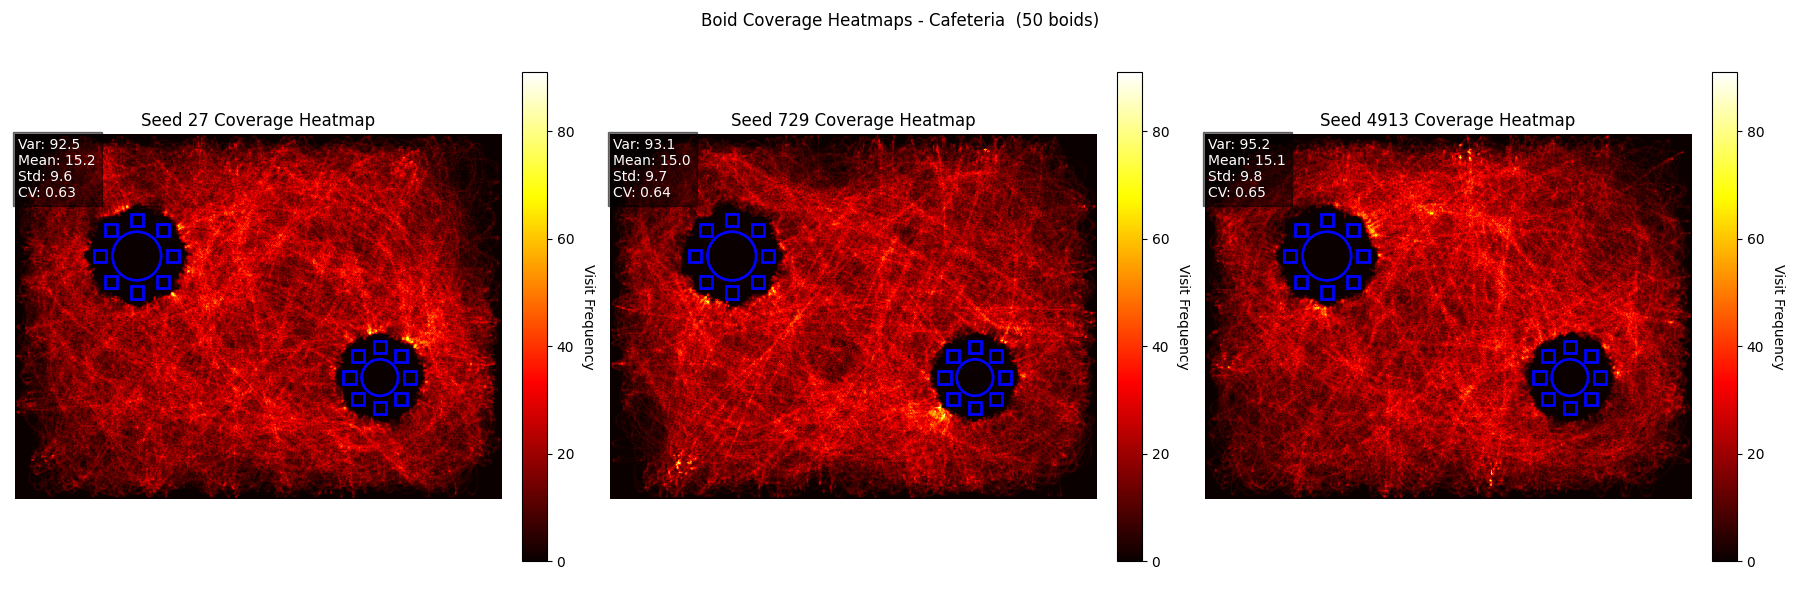
\includegraphics[width=\linewidth]{heatmaps/cafeteria_50.png}
    \caption{Coverage heatmap for the Cafeteria map with $N=50$ boids.}
    \label{fig:app:caf50_heat}
  \end{subfigure}
  \caption{Coverage analysis for the Cafeteria environment with $N=50$ boids: (a) relationship between behavioral gains and coverage, (b) cumulative coverage over time, (c) visitation frequency heatmap.}
  \label{fig:app:cafeteria50}
\end{figure}

%----------------------------------------------------------------
% Dense Cafeteria, N = 50
\begin{figure}[h!]
  \centering
  \begin{subfigure}[b]{0.32\linewidth}
    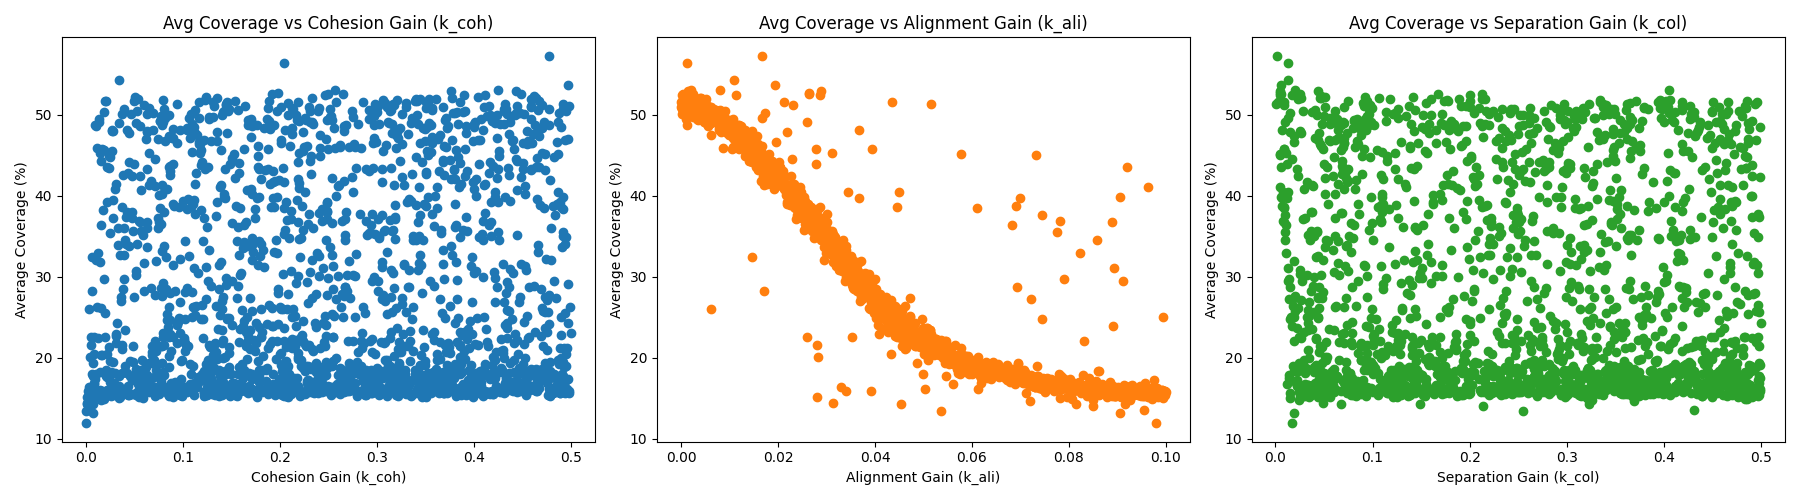
\includegraphics[width=\linewidth]{cov_vs_gains/dense_50.png}
    \caption{Coverage vs.~gains for the Dense Cafeteria map with $N=50$ boids.}
    \label{fig:app:dense50_gains}
  \end{subfigure}\hfill
  \begin{subfigure}[b]{0.32\linewidth}
    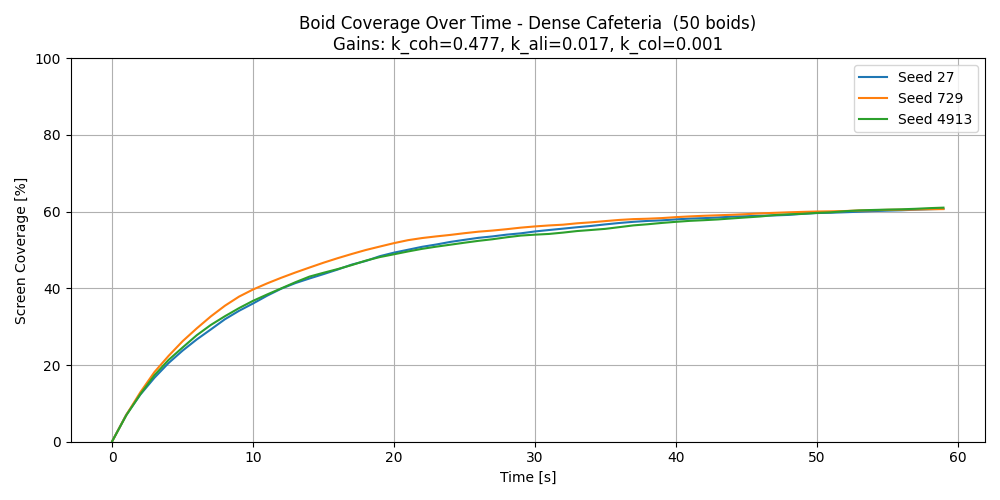
\includegraphics[width=\linewidth]{optimal_cov_vs_time/dense_50.png}
    \caption{Coverage over time for the Dense Cafeteria map with $N=50$ boids.}
    \label{fig:app:dense50_time}
  \end{subfigure}\hfill
  \begin{subfigure}[b]{0.32\linewidth}
    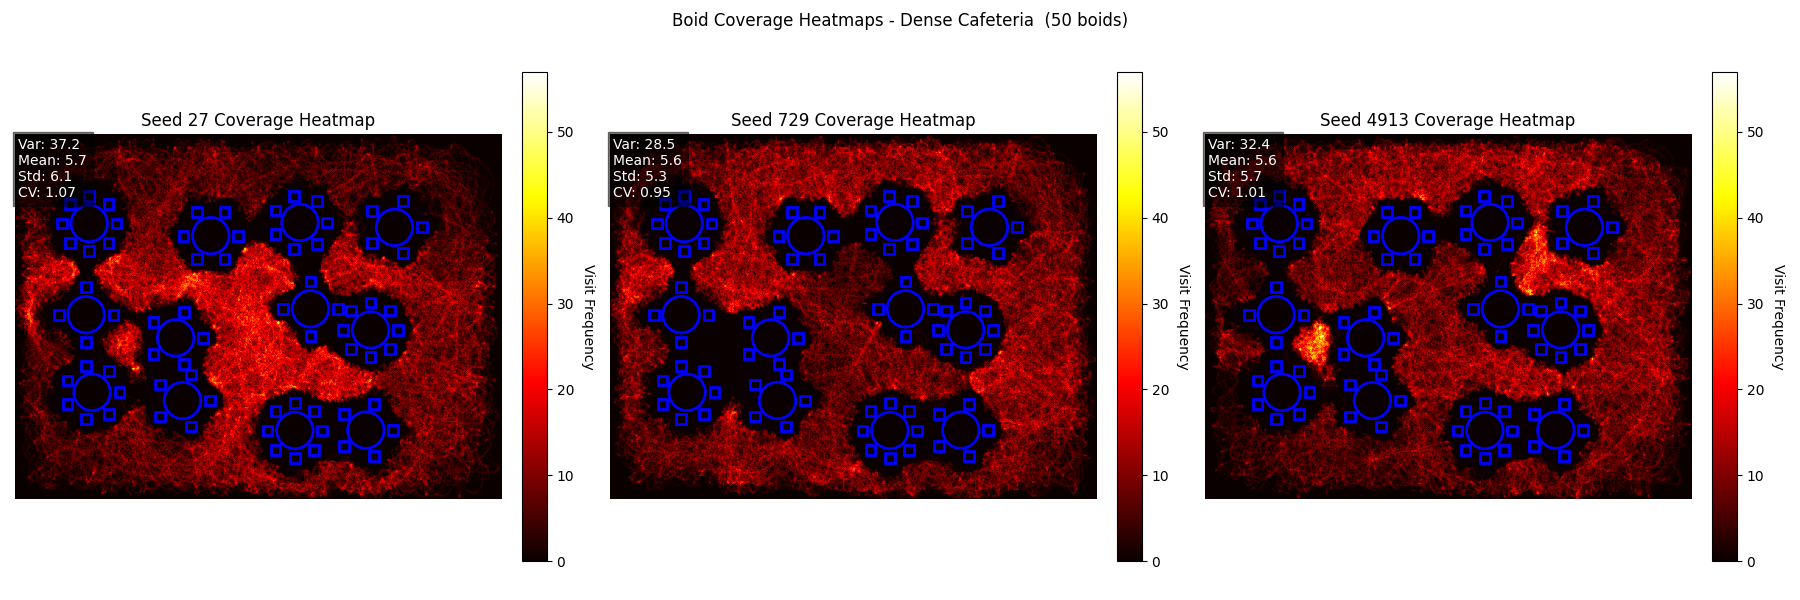
\includegraphics[width=\linewidth]{heatmaps/dense_50.png}
    \caption{Coverage heatmap for the Dense Cafeteria map with $N=50$ boids.}
    \label{fig:app:dense50_heat}
  \end{subfigure}
  \caption{Coverage analysis for the Dense Cafeteria environment with $N=50$ boids: (a) coverage vs.~gains, (b) cumulative coverage over time, (c) coverage heatmap.}
  \label{fig:app:densecaf50}
\end{figure}

%----------------------------------------------------------------
% Dense Cafeteria, N = 100
\begin{figure}[h!]
  \centering
  \begin{subfigure}[b]{0.32\linewidth}
    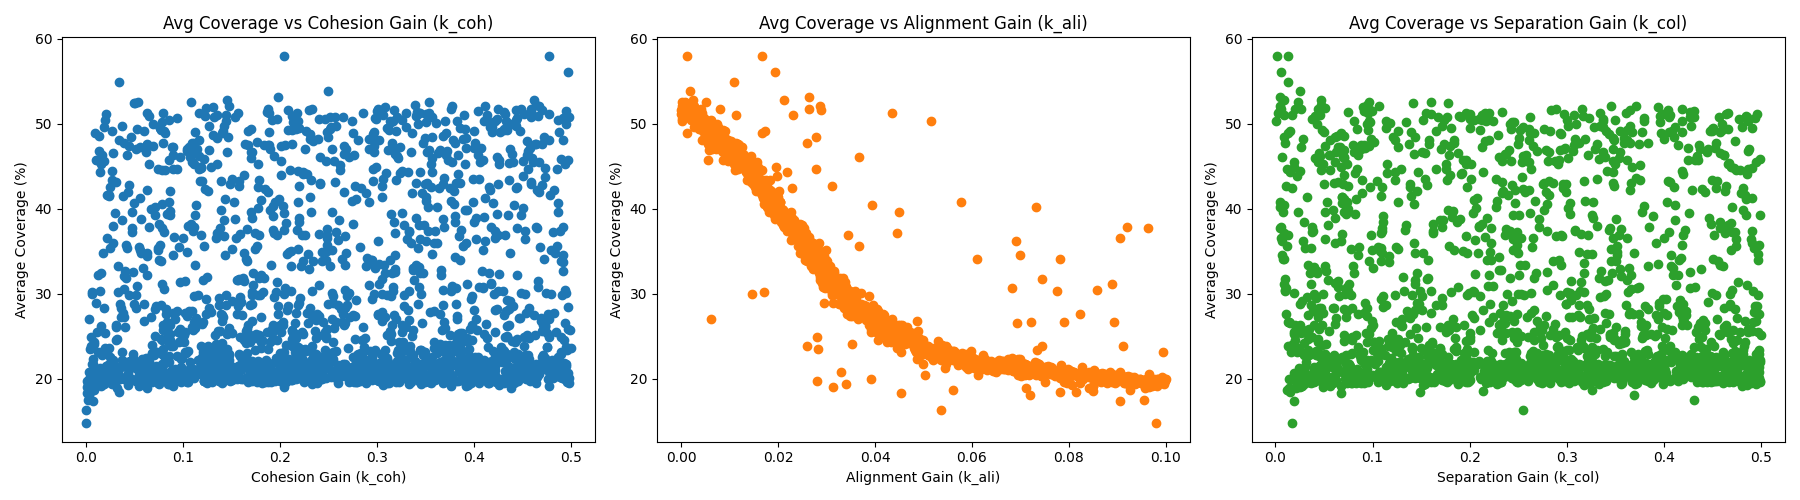
\includegraphics[width=\linewidth]{cov_vs_gains/dense_100.png}
    \caption{Coverage vs.~gains for the Dense Cafeteria map with $N=100$ boids.}
    \label{fig:app:dense100_gains}
  \end{subfigure}\hfill
  \begin{subfigure}[b]{0.32\linewidth}
    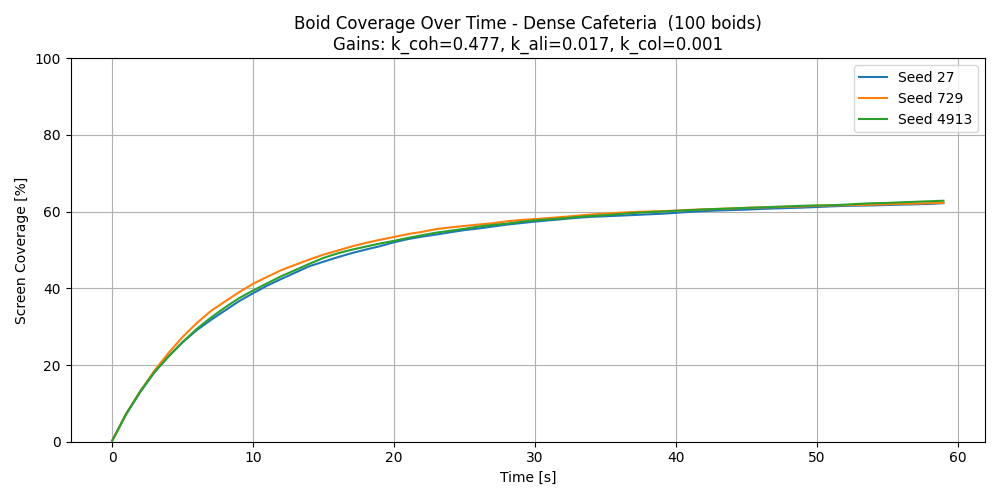
\includegraphics[width=\linewidth]{optimal_cov_vs_time/dense_100.png}
    \caption{Coverage over time for the Dense Cafeteria map with $N=100$ boids.}
    \label{fig:app:dense100_time}
  \end{subfigure}\hfill
  \begin{subfigure}[b]{0.32\linewidth}
    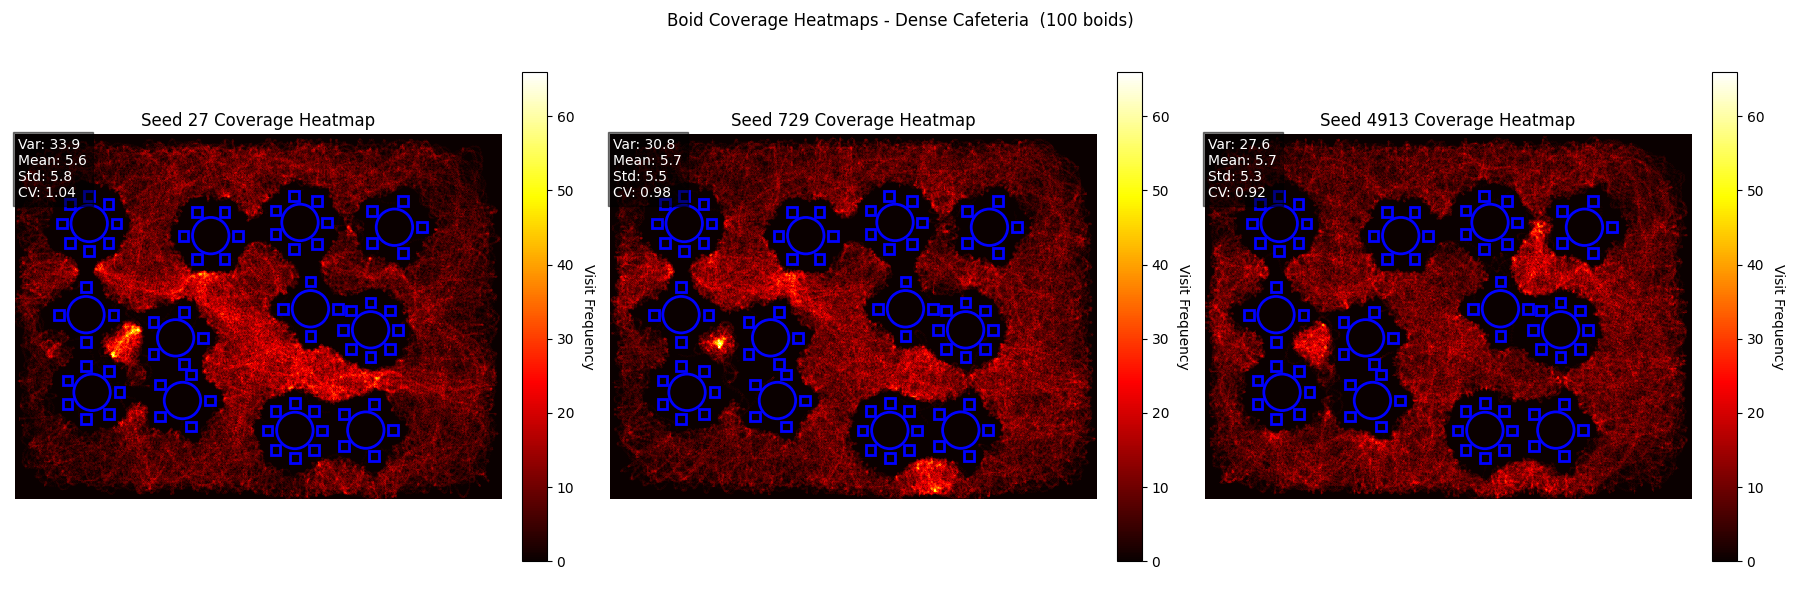
\includegraphics[width=\linewidth]{heatmaps/dense_100.png}
    \caption{Coverage heatmap for the Dense Cafeteria map with $N=100$ boids.}
    \label{fig:app:dense100_heat}
  \end{subfigure}
  \caption{Coverage analysis for the Dense Cafeteria environment with $N=100$ boids: (a) coverage vs.~gains, (b) cumulative coverage over time, (c) coverage heatmap.}
  \label{fig:app:densecaf100}
\end{figure}

%----------------------------------------------------------------
% Empty Map, N = 50
\begin{figure}[h!]
  \centering
  \begin{subfigure}[b]{0.32\linewidth}
    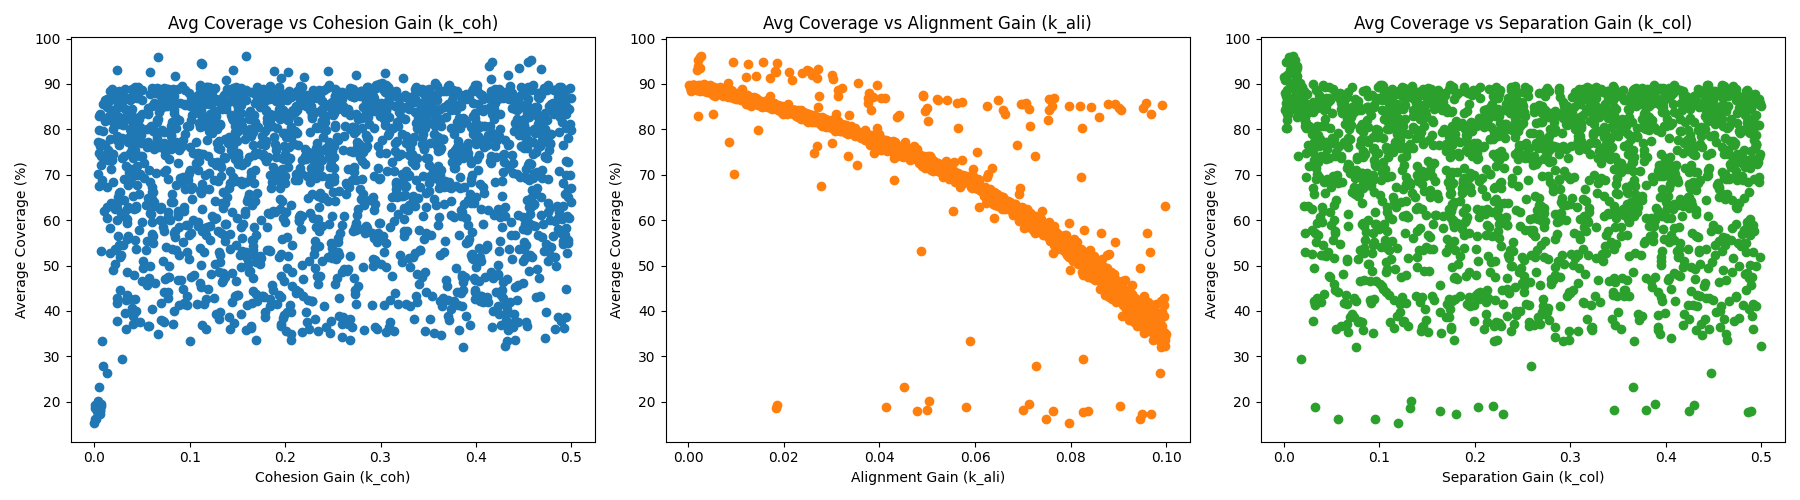
\includegraphics[width=\linewidth]{cov_vs_gains/empty_50.png}
    \caption{Coverage vs.~gains for the Empty map with $N=50$ boids.}
    \label{fig:app:empty50_gains}
  \end{subfigure}\hfill
  \begin{subfigure}[b]{0.32\linewidth}
    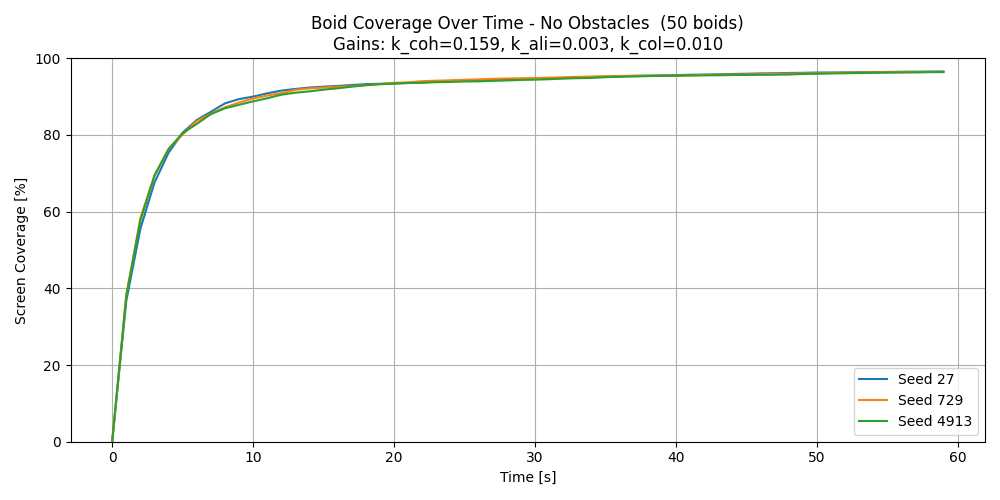
\includegraphics[width=\linewidth]{optimal_cov_vs_time/empty_50.png}
    \caption{Coverage over time for the Empty map with $N=50$ boids.}
    \label{fig:app:empty50_time}
  \end{subfigure}\hfill
  \begin{subfigure}[b]{0.32\linewidth}
    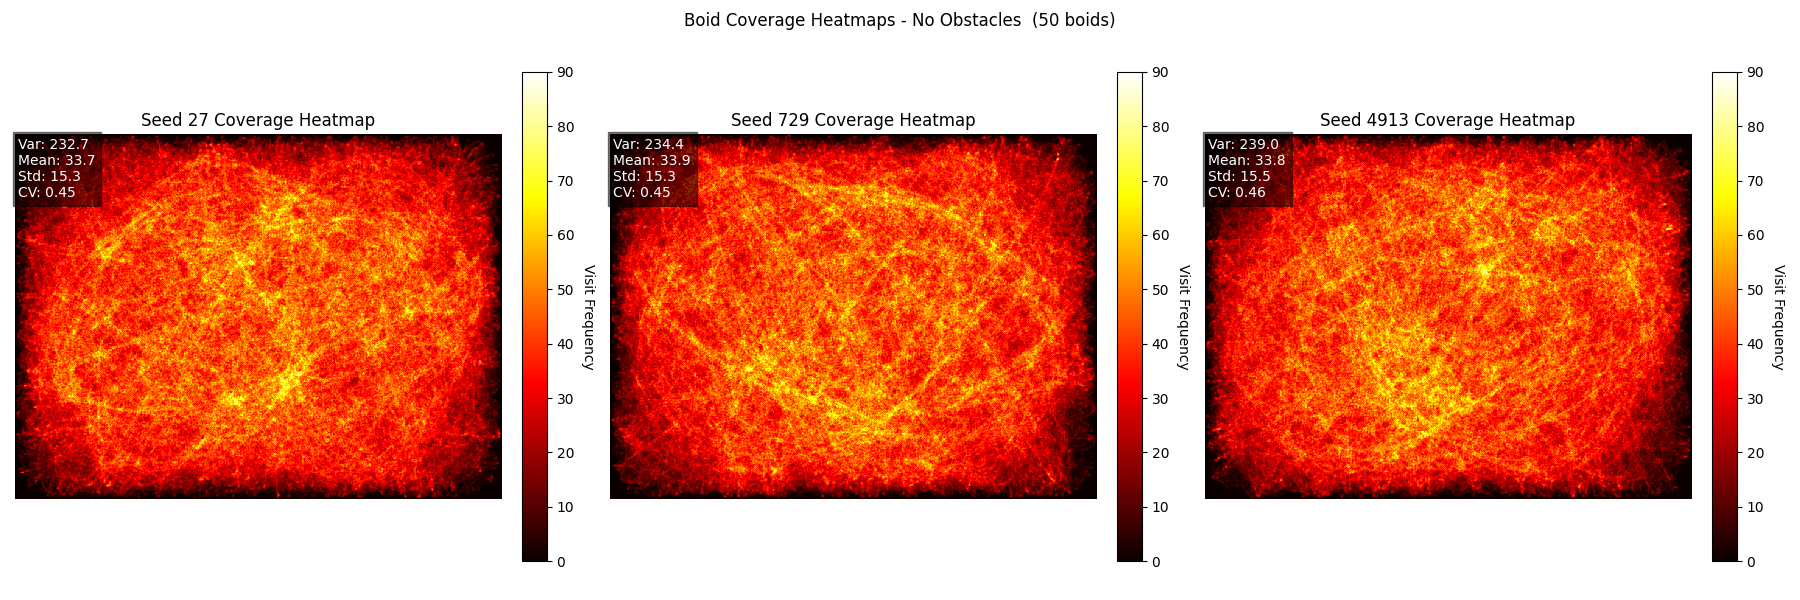
\includegraphics[width=\linewidth]{heatmaps/empty_50.png}
    \caption{Coverage heatmap for the Empty map with $N=50$ boids.}
    \label{fig:app:empty50_heat}
  \end{subfigure}
  \caption{Coverage analysis for the Empty environment with $N=50$ boids: (a) coverage vs.~gains, (b) cumulative coverage over time, (c) coverage heatmap.}
  \label{fig:app:empty50}
\end{figure}

%----------------------------------------------------------------
% Empty Map, N = 100
\begin{figure}[h!]
  \centering
  \begin{subfigure}[b]{0.32\linewidth}
    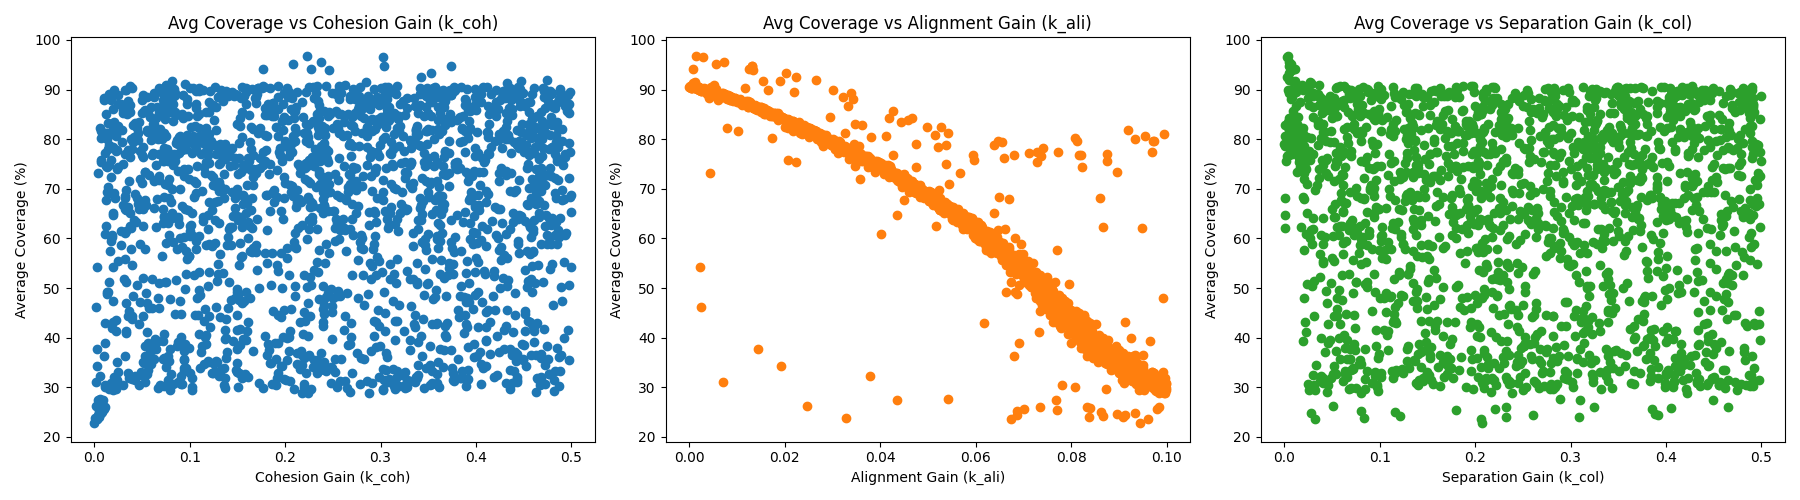
\includegraphics[width=\linewidth]{cov_vs_gains/empty_100.png}
    \caption{Coverage vs.~gains for the Empty map with $N=100$ boids.}
    \label{fig:app:empty100_gains}
  \end{subfigure}\hfill
  \begin{subfigure}[b]{0.32\linewidth}
    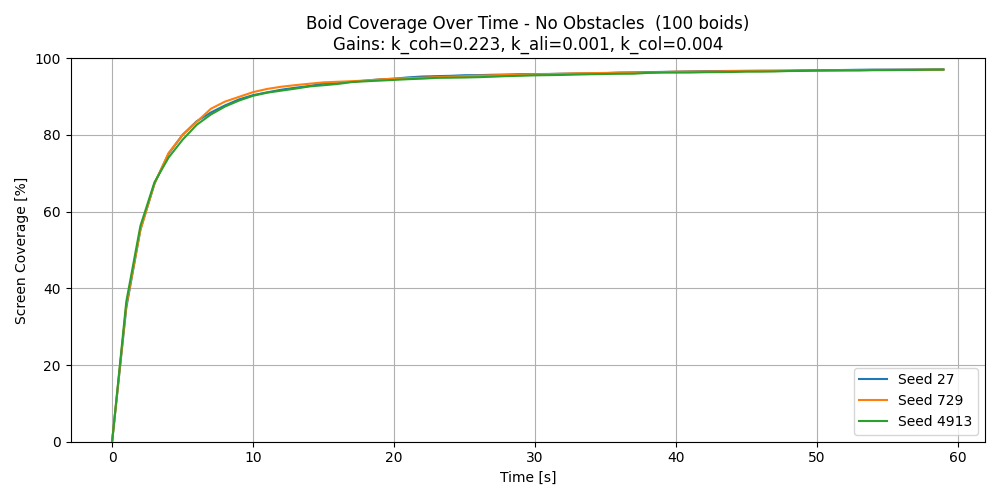
\includegraphics[width=\linewidth]{optimal_cov_vs_time/empty_100.png}
    \caption{Coverage over time for the Empty map with $N=100$ boids.}
    \label{fig:app:empty100_time}
  \end{subfigure}\hfill
  \begin{subfigure}[b]{0.32\linewidth}
    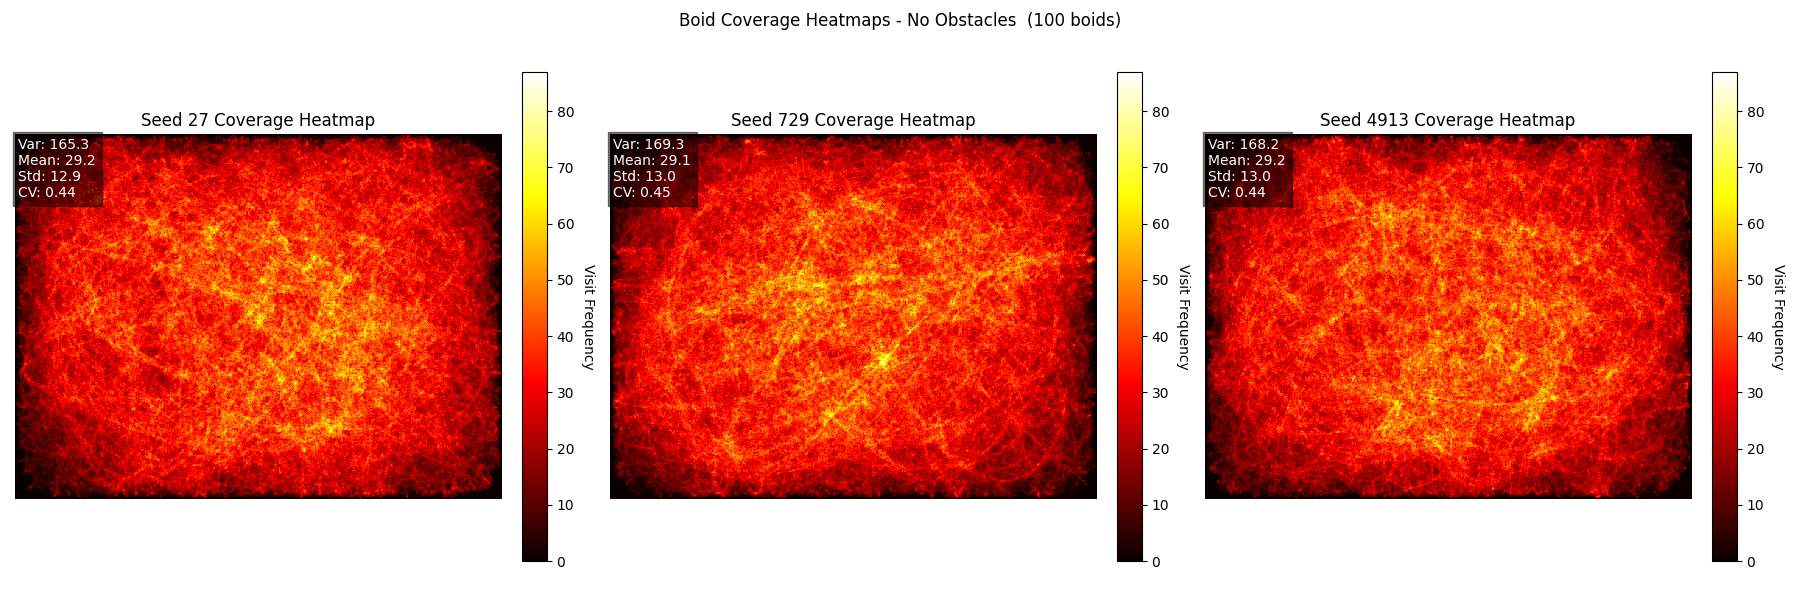
\includegraphics[width=\linewidth]{heatmaps/empty_100.png}
    \caption{Coverage heatmap for the Empty map with $N=100$ boids.}
    \label{fig:app:empty100_heat}
  \end{subfigure}
  \caption{Coverage analysis for the Empty environment with $N=100$ boids: (a) coverage vs.~gains, (b) cumulative coverage over time, (c) coverage heatmap.}
  \label{fig:app:empty100}
\end{figure}

%----------------------------------------------------------------
% Narrow Corridor, N = 50
\begin{figure}[h!]
  \centering
  \begin{subfigure}[b]{0.32\linewidth}
    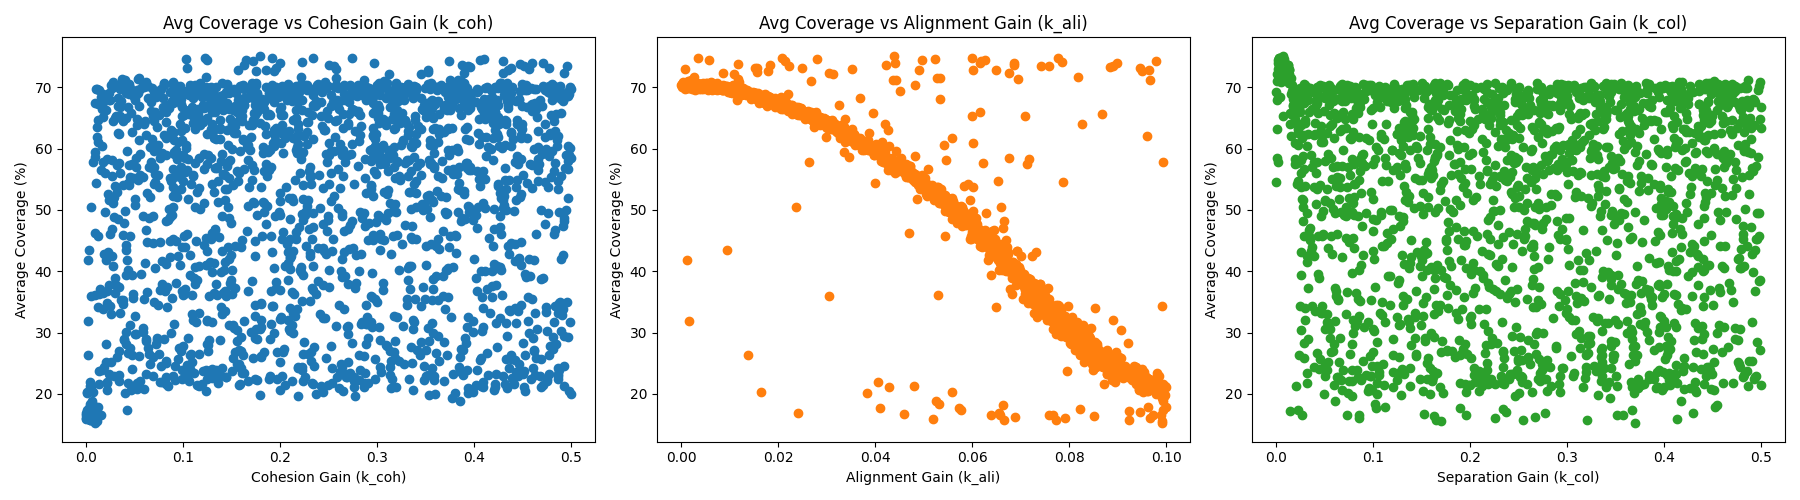
\includegraphics[width=\linewidth]{cov_vs_gains/narrow_50.png}
    \caption{Coverage vs.~gains for the Narrow Corridor map with $N=50$ boids.}
    \label{fig:app:narrow50_gains}
  \end{subfigure}\hfill
  \begin{subfigure}[b]{0.32\linewidth}
    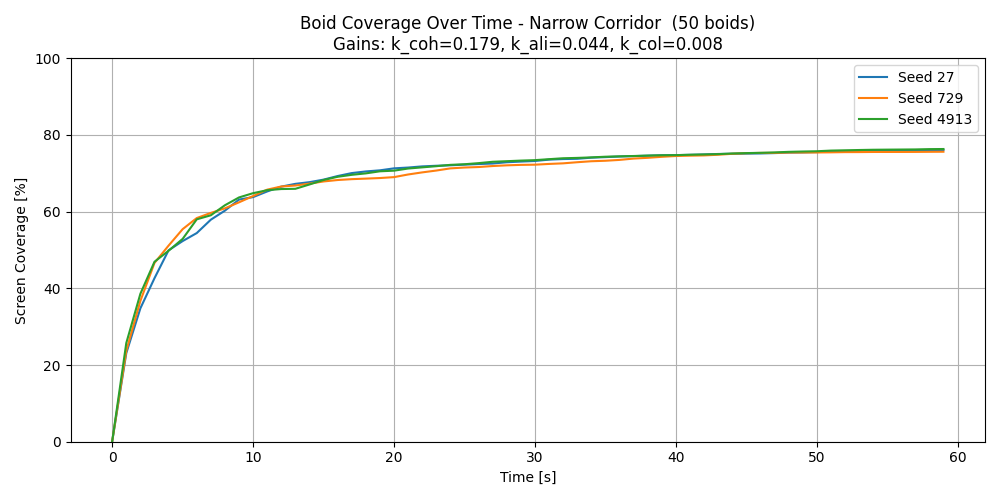
\includegraphics[width=\linewidth]{optimal_cov_vs_time/narrow_50.png}
    \caption{Coverage over time for the Narrow Corridor map with $N=50$ boids.}
    \label{fig:app:narrow50_time}
  \end{subfigure}\hfill
  \begin{subfigure}[b]{0.32\linewidth}
    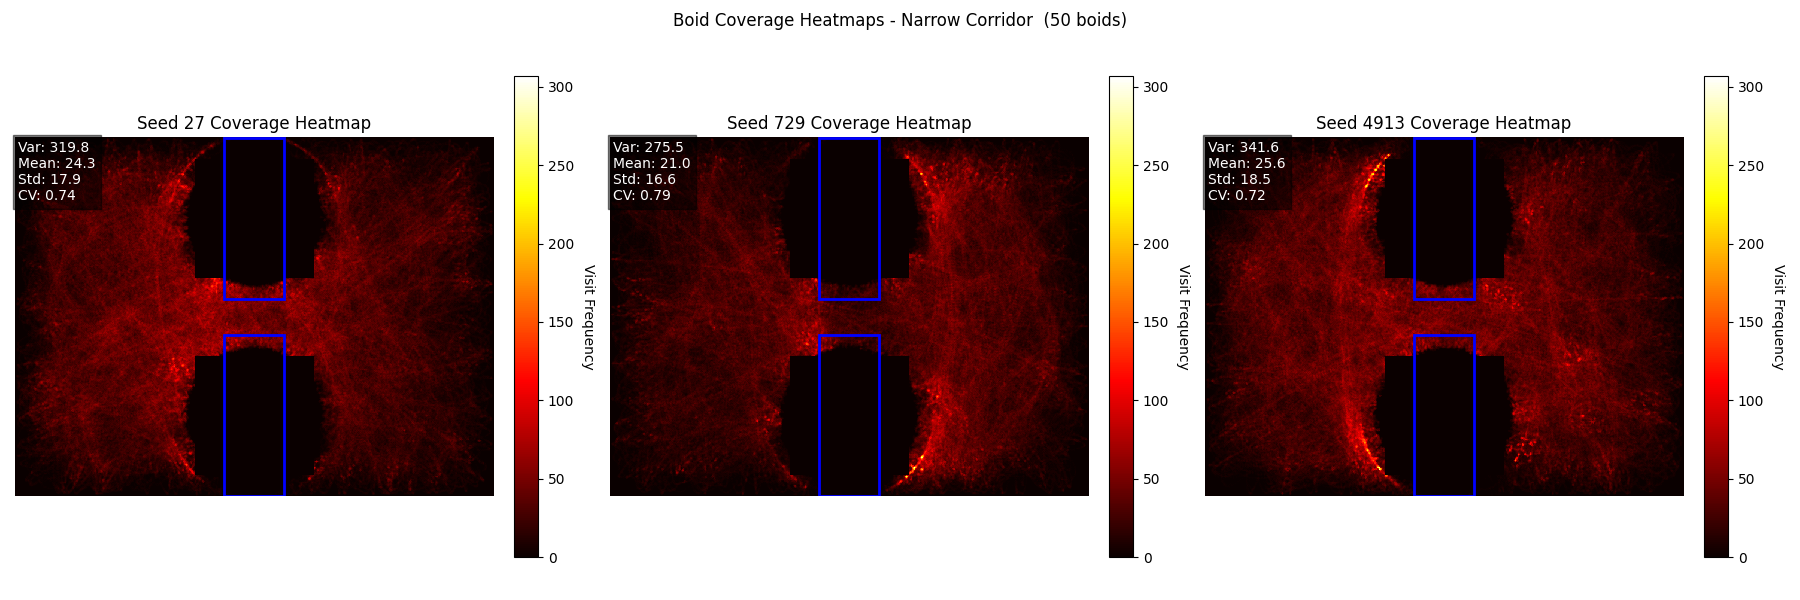
\includegraphics[width=\linewidth]{heatmaps/narrow_50.png}
    \caption{Coverage heatmap for the Narrow Corridor map with $N=50$ boids.}
    \label{fig:app:narrow50_heat}
  \end{subfigure}
  \caption{Coverage analysis for the Narrow Corridor environment with $N=50$ boids: (a) coverage vs.~gains, (b) cumulative coverage over time, (c) coverage heatmap.}
  \label{fig:app:narrow50}
\end{figure}

%----------------------------------------------------------------
% Narrow Corridor, N = 100
\begin{figure}[h!]
  \centering
  \begin{subfigure}[b]{0.32\linewidth}
    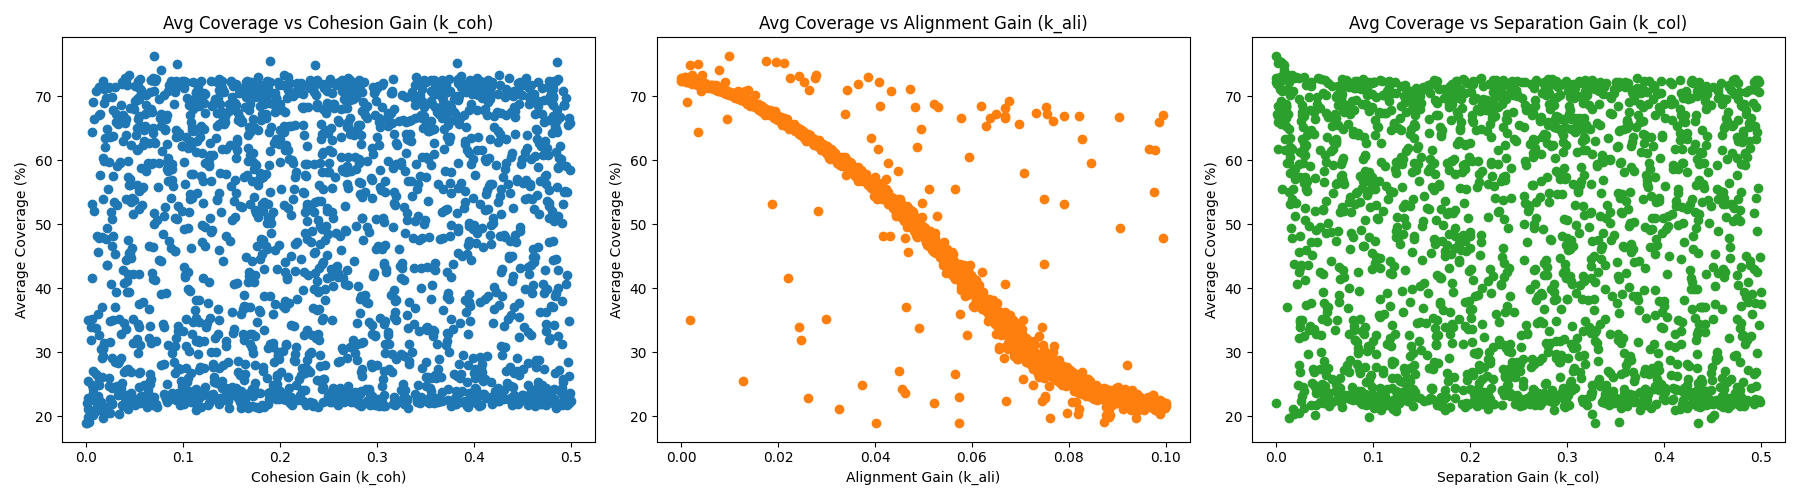
\includegraphics[width=\linewidth]{cov_vs_gains/narrow_100.png}
    \caption{Coverage vs.~gains for the Narrow Corridor map with $N=100$ boids.}
    \label{fig:app:narrow100_gains}
  \end{subfigure}\hfill
  \begin{subfigure}[b]{0.32\linewidth}
    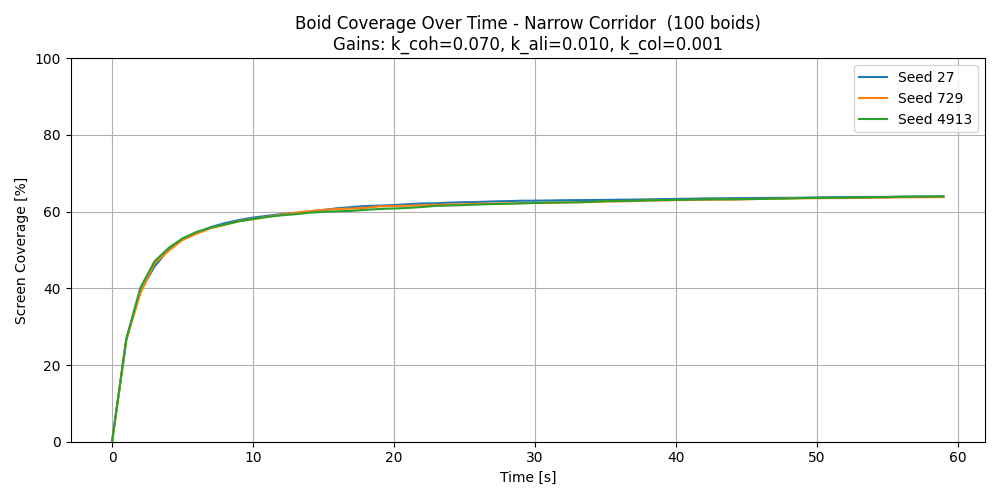
\includegraphics[width=\linewidth]{optimal_cov_vs_time/narrow_100.png}
    \caption{Coverage over time for the Narrow Corridor map with $N=100$ boids.}
    \label{fig:app:narrow100_time}
  \end{subfigure}\hfill
  \begin{subfigure}[b]{0.32\linewidth}
    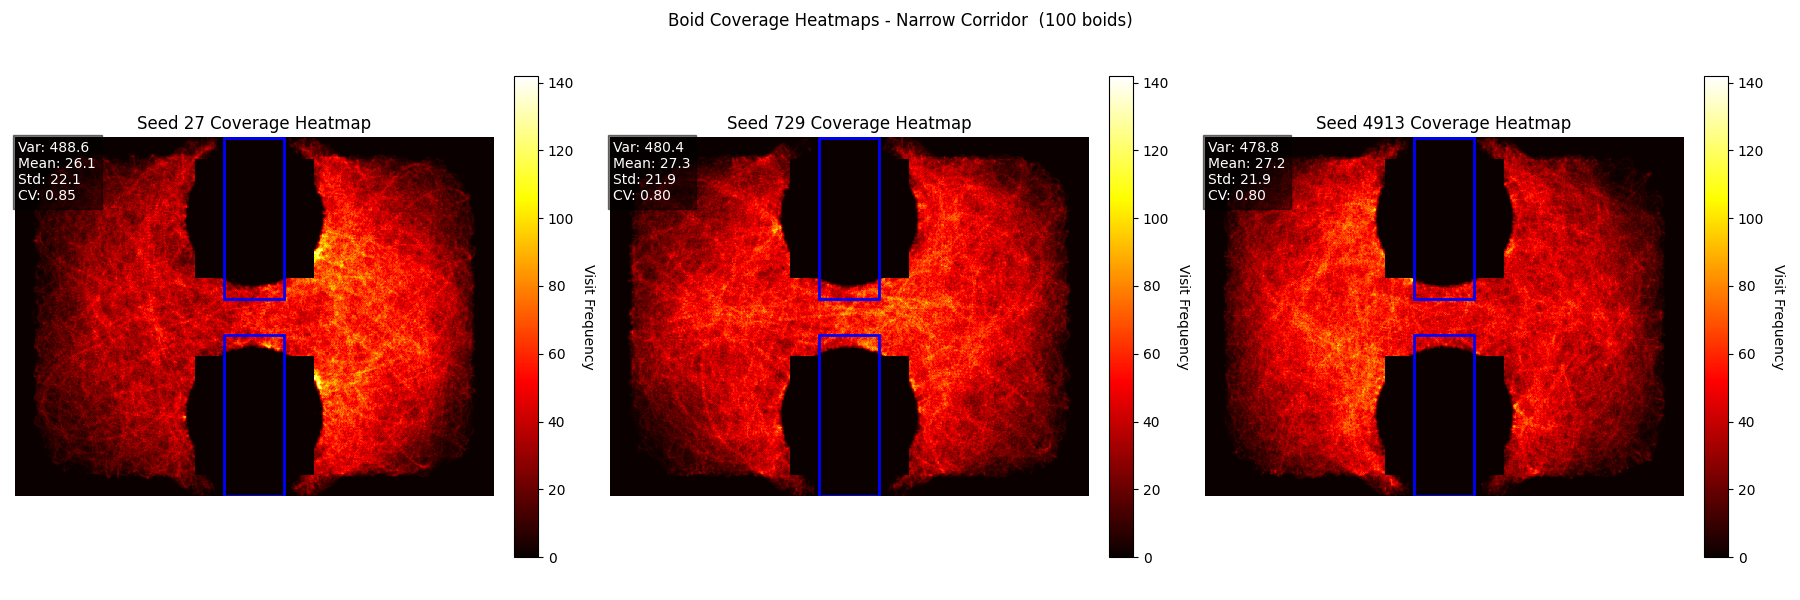
\includegraphics[width=\linewidth]{heatmaps/narrow_100.png}
    \caption{Coverage heatmap for the Narrow Corridor map with $N=100$ boids.}
    \label{fig:app:narrow100_heat}
  \end{subfigure}
  \caption{Coverage analysis for the Narrow Corridor environment with $N=100$ boids: (a) coverage vs.~gains, (b) cumulative coverage over time, (c) coverage heatmap.}
  \label{fig:app:narrow100}
\end{figure}


\end{document}
